\documentclass[12pt,a4paper]{article}
\usepackage{lscape}
\usepackage{pdflscape, adjustbox}
\usepackage[para,online,flushleft]{threeparttable}
\usepackage{amsmath,hyperref,amsfonts,caption,subcaption,graphicx,float,chngcntr,booktabs,array,lscape}
\usepackage{graphicx}
\usepackage{longtable}
\usepackage{longtable}
\usepackage{adjustbox} 
\usepackage[a4paper, total={6in, 10in}]{geometry}
\usepackage{comment}
 \usepackage{multirow}
% Continuous Fig numbers
\counterwithin{figure}{section}
\counterwithin{table}{section}
% Reference hyperlink color
\hypersetup{
    colorlinks=true,
    linkcolor=blue,
    citecolor=blue,
    filecolor=magenta,      
    urlcolor=cyan,
    pdftitle={Research Proposal},
    pdfpagemode=FullScreen}
% Font
\usepackage[T1]{fontenc}
\usepackage{tgpagella}
\usepackage{natbib}
\usepackage{tabularx} 
\usepackage[dvipsnames]{xcolor}
\usepackage{enumitem}
\usepackage{subcaption}
%% APA style
\bibliographystyle{elsarticle-harv}
%\biboptions{authoryear,square,comma}
\makeatletter

% Optional: Uncomment and adjust if you need Persian support
%\usepackage{xepersian}
%\settextfont{XB Niloofar}

% Article metadata
\title{Poverty Dynamics in Iran: Substitutes for Missing Data\thanks{We sincerely thank our colleagues at the Graduate School of Management and Economics (GSME) for their critical engagement during our weekly seminar series. Our gratitude also extends to the International Iranian Economic Association (IIEA) monthly webinar participants, and attendees in the XXX} }

\author{GholamReza Keshavarz Haddad\thanks{(Corresponding Author) Associate Professor, GSME, Sharif University of Technology. ORCID: 0000-0001-5873-8217, Email: G.K.Haddad@sharif.edu} \and Ahmad MohammadZadeh \thanks{Researcher, GSME, Sharif University of Technology. Email: ahmad.mohamadzadeh@gmail.com} \and XX \thanks{ZZ} }
\date{\today} % Leave empty to omit the date or specify if needed

\begin{document}

\maketitle

 %‎\renewcommand{\baselinestretch}{1.7}
 %\footnotesize{
\begin{abstract}
\noindent
\textbf{Objective:} Measuring poverty dynamics---distinguishing chronic from transient poverty---is crucial for effective anti-poverty policies, yet constrained by limited panel data in developing countries.

\textbf{Method:} We overcome this constraint by constructing a synthetic panel from the Iranian Household Expenditure and Income Survey (HIES). Using a consumption model, we estimate first-round consumption for households only observed in the second round, enabling dynamic poverty analysis despite the absence of true longitudinal data.

\textbf{Findings:} Our analysis for 1398-1399 reveals that 29\% of households were chronically poor (poor in both years). Chronic poverty is markedly higher among vulnerable subgroups: 54\% in rural households, 40\% in female-headed households, and 34\% in households with non-university educated heads. Notably, our synthetic panel estimates consistently encompass the true panel values where available, validating the method's reliability.

\textbf{Conclusion:} Synthetic panels provide a viable alternative for tracking poverty transitions where traditional panel data are absent, revealing significant heterogeneities that warrant targeted policy attention.
\begin{comment}
    Eliminating poverty, which is one of the most important objectives of countries, requires a deep understanding of the trends and dynamics of poverty and the distinction between chronic and transient poverty.
However, given the lack of high-quality panel data, measuring movements in and out of poverty in developing countries is difficult. In this research, we build a synthetic panel by constructing a consumption model
and estimating the first-round consumption of households surveyed in the second round. The analysis of Expenditures and Income Survey (HIES) for 1398 and 1399 shows that almost 29 percent of urban and rural
households were poor in both years. In female-headed households, households with non-university educated
heads, and rural households, this rate is 40, 34, and 54 percent, respectively, indicating their need for special
attention. Moreover, the results of the synthetic panel virtually always include the true panel estimates.

\end{comment}
\smallskip

\noindent \textbf{Keywords:} chronic and transient poverty, poverty dynamics, synthetic panel data\\
\textbf{JEL Classification:} XX; YY; ZZ
\end{abstract}


% \mykeyword{chronic and transient poverty, poverty dynamics, synthetic panel data}
%\newpage
	
\section{Introduction}
Eradicating poverty is a crucial objective for nations worldwide, with the United Nations committing to "ending poverty in all its forms everywhere" as one of its sustainable goals. However, the COVID-19 pandemic has impeded progress towards this goal, resulting in an increase in the global rate of extreme poverty for the first time in over two decades and an additional 120 million people living in poverty in 2020\footnote{\url{https://sdgs.un.org/goals/goal1}}.

The World Bank's standardized international poverty line—set at \$8.3 per person per day in 2021 Purchasing Power Parity (PPP) exchange rates—has been customized for several nations, including Iran \citep{worldbank2026iran}. It is designed specifically to measure poverty at higher income levels and is particularly relevant for the economic context of upper-middle-income countries \citep{Ferreira2016}. This measure is a part of a larger tiered analytical framework that includes the revised extreme poverty line (\$3.00) and a lower-middle-income line (\$4.15), providing a multi-lens view of global deprivation, \citep{Jolliffe2022}. 

%\subsection{Engel Coefficient}
In addition to the World Bank's poverty thresholds, a well-documented alternative approach to calculating the poverty headcount ratio uses the food expenditure share exceeding 50\% of total consumption. This method is grounded in Engel's Law, which posits that as household income increases, the share of expenditure devoted to food declines \citep{Engel1857}. A share above 50\% signals that a household is allocating the majority of its resources to basic subsistence, leaving little for other essential needs such as healthcare, education, and shelter \citep{Ravallion1992, Ravallion2011}. This indicator is behaviorally grounded, relatively inflation-resistant, and useful for cross-sectional and historical comparisons, especially in low-income settings \citep{Deaton1997}.

\begin{figure}[!htb]
   \caption{Headcount Ratio, by Area of Residence}
    \includegraphics[width=0.95\linewidth]{"Figures/PovLines"}
    \caption*{\scriptsize \textbf{Note:} LMICs and UMICs stand for lower-middle-income and upper-middle-income countries, respectively. All of the poverty lines reveal a quite similar trend for the population under the poverty line; however, the level of the lower-middle-income poverty line is arguably lower than the Engel coefficient and that for upper-middle-income countries. We use the consumption PPP converter produced by the World Bank, which is based on 2021 fixed prices. The gray vertical lines refer to presidential election years. The highest poverty rate was realized during Hashemi Rafsanjani's presidential administration, in the year that CPI growth exceeded 49 percent and triggered the first social unrest in some cities since the 1998 Islamic Revolution.\\
    Source: HIES 1991-2024 for food, non-food and househols' size, and world bank for PPP converter.}
    \label{fig:placeholder}
\end{figure}
However, its application has significant limitations. It does not account for demographic differences, shifts in food quality, or the growing importance of non-food necessities in modern economies \citep{Lipton1988, Banerjee2011}. Consequently, while informative, the 50\% threshold is best employed as one component within a broader multidimensional poverty assessment, rather than as a standalone measure \citep{Alkire2011, WorldBank2017}. 
\autoref{fig:placeholder} plots the  headcount ratio trends by region, level of poverty line upper-Middle-Income Countries (8.3 PPP),  Lower-Middle-Income Countries (4.15 PPP) and the headcount ratio based on food expenditures over 50\% of total monthly expenditures.  The patterns of the trends are very similar and almost decreasing, although after the US exit from the JCPOA, the headcount ratio turned to exhibit increasing trend. The poverty rate in Rural areas is significantly higher than urban areas and in 2010 it reached to the highest level of about 50\% in terms of 8.0 PPP exchange rate.\par

The utilization of the \$8.0 per day poverty line—the global benchmark for Upper-Middle-Income Countries (UMICs)—often yields significantly elevated poverty headcount ratios in rural contexts, suggesting a critical disconnect between the uniform international standard and local cost-of-living heterogeneity. This discrepancy is largely attributed to the non-application of intra-country spatial price deflators, which fail to account for systematic differences in the cost of a basic needs basket between urban and rural areas \citep{chen2020, dabalen2019}. Furthermore, the overestimation of rural poverty is compounded by the challenge of accurately valuing non-monetary consumption—specifically, own-produced food consumed by subsistence and semi-subsistence farming households—which is a major component of real welfare in rural UMICs yet is frequently undervalued or inconsistently measured in household surveys \citep{ravallion2008}. \\
\begin{comment}
While the World Bank has advanced a Societal Poverty Line (SPL)---defined as
$$\text{SPL} = \max\{\$2.15 \text{ PPP}, \$1.15 + 0.5 \times \text{Median Consumption} \}$$


 \par
to introduce a relative component that reflects rising consumption standards, the absolute \$6.85 line itself, derived from the median of UMIC national lines, acts as a high poverty threshold that can dramatically exceed the actual national SPL for many UMICs, resulting in a structurally high poverty count that may overstate deprivation relative to locally accepted minimum living standards, \cite{Jolliffe2022AssessingTI}. 

Consequently, researchers advocate for sub-national poverty estimates that incorporate region-specific price indices and rigorously impute the value of auto-consumption to align international measures with localized welfare realities, \cite{deaton2002, worldbank2024}.



In Iran, the poverty rate was reported ( \textcolor{red}{Which poverty rate? whole country? Based on which poverty line?} )as 16\% in 2017, with unofficial statistics indicating a significant increase since then, \citep{majlis1398poverty}.
\end{comment}
%%%%%%%%%%%%%%%%%%%%%%%
Static poverty profiles  and or national trends provide only a snapshot, conflating chronic and transitory poverty while obscuring welfare trajectories, duration, and vulnerability - limitations that undermine effective targeting \cite{BaulchHoddinott2000}. Dynamic presentations, by contrast, disaggregate the poor into distinct groups, identify drivers of poverty transitions, assess policy effectiveness, and reveal risk and persistence \cite{BarrettCarter2016}. This richer understanding enables differentiated, evidence-based interventions that address both immediate needs and long-term structural vulnerabilities, making dynamic analysis indispensable for effective poverty reduction strategies \cite{CarterBarrett2006, Dercon2005, HulmeShepherd2003}.
The shift from examining static poverty profiles or national trends to analyzing poverty dynamics constitutes a crucial methodological and theoretical advance in development economics and social policy. For our study of Iran, this transition to a dynamic perspective provides a richer understanding necessary for effective, targeted intervention. The core argument rests on the fact that poverty is an inherently heterogeneous and time-varying living circumstance \citep{BaulchHoddinott2000}. Static analyses, typically derived from cross-sectional data, capture only a snapshot in time and are inherently limited in addressing the processes that determine an individual's or household's welfare trajectory. By contrast, a dynamic approach—relying on longitudinal (panel) data—allows for the disaggregation of the poor population into distinct sub-groups that static measures conflate \citep{BarrettCarter2016}. The most significant conceptual contribution of poverty dynamics is the distinction between chronic and transitory poverty \citep{HulmeShepherd2003}.

 Households or individuals who remain below the poverty line for an extended period—often across multiple survey waves—are classified as chronically poor. This group is typically trapped by long lasting structural challenges and limited asset endowments. In the Iranian context, for example, persistently high inflation, structural unemployment, and a low minimum wage (760 international PPP dollars per month, based on the implied PPP conversion rate of 289,230 for 2026) may be driving an increase in chronic poverty, as recent analyses suggest \citep{EslamiHoseini2024}. Households with transitory poverty move into and out of poverty, often due to temporary income shocks, such as illness, job loss, climate-related events (like floods), or volatile price fluctuations.\par
Policy prescriptions differ fundamentally for these two groups. Poverty alleviation strategies that rely on static data are inherently limited, as they apply generic interventions to a heterogeneous population, overlooking the distinct needs of chronic versus transitory poor.\par

 A dynamic perspective enables scholars and policymakers to quantify and analyze vulnerability to poverty \citep{ChaudhuriJalanSuryahadi2002}. This forward-looking metric identifies non-poor households that face a high risk of falling into poverty due to future shocks. Analyzing vulnerability is essential for designing preventative rather than purely reactive policy. In an environment like Iran—characterized by macroeconomic volatility, high inflation, and devastating sanctions \citep{WorldBank2023}-understanding which households are vulnerable, particularly those in the shrinking middle class, becomes critically important for preventing a broader social catastrophe. Static analysis can only identify correlates of poverty, such as household size or the education level of the head. By contrast, dynamic analysis reveals the specific events and processes—the drivers—that cause households to transition into or out of poverty \citep{McKayOkidi2003}. To avoid inclusion and exclusion errors—and to ensure efficient use of limited resources—policymakers must distinguish between transient and chronic poverty, a task that requires dynamic analysis \citep{dang2020impute, baulch2000economic}.
 
 %Using econometric techniques like logit or probit models on panel data, one can determine:The probability of exit from poverty (e.g., driven by increased returns to education or formal sector employment).The probability of entry into poverty (e.g., driven by illness, death of a wage earner, or covariate shocks like severe inflation or natural disasters).This provides actionable intelligence for policymakers. For instance, if entry is strongly linked to health shocks, policy attention should shift to providing effective health insurance.
%%%%%%%%%%%%%%%%%%%%%%%%%%%%%%%%%%%
%To effectively address poverty, policymakers must engage in a process of accurate evaluation and observation, as there are a variety of policy options available, ranging from short-term support for families at risk of poverty to long-term measures such as investment in education and skill training through achieving economic growth. To prevent inefficient use of limited resources, it is crucial to understand trends and dynamics of poverty, and distinguish between transient and chronic poverty \citep{dang2020impute}. Static measures of poverty can lead to inclusion and exclusion errors, as policymakers may mistakenly provide resources to individuals who are not actually poor, but experiencing temporary financial hardships, or fail to provide support to poor families experiencing short-term favorable circumstances. Analysis of poverty dynamics can assist policymakers in designing safety net policies to protect vulnerable households and gain a better understanding of factors that contribute to economic mobility \citep{baulch2000economic}.

 
Measuring movements in and out of poverty, particularly in developing countries, is a challenging task due to the lack of panel data, which is the most appropriate source of information. However, there is a growing body of literature that has developed techniques to measure poverty dynamics in the absence of panel data \citep{cruces2015estimating}. \par

This paper seeks to estimate poverty transitions in Iran using the "synthetic panel" method developed by \citep{dang2014using}, based on Expenditures and Income surveys taken in 2019 and 2020. These years are particularly important due to the severity of sanctions against Iran and the outbreak of the coronavirus. The synthetic panel method produces lower and upper bound estimates of poverty transitions, which are expected to sandwich true poverty transition estimates.\par
This paper is the first that validates the synthetic panel approach for a developing country under sanctions, and the results indicate that the lower and upper bounds fully encompass the true poverty dynamic measures in most cases. Additionally, the results show that almost 29\% of urban and rural households were poor in both years, with higher rates in female-headed households, households with non-university educated heads, and rural households, indicating a need for special attention in these groups.\par
The rest of the paper is organized as follows. Section two outlines the underlying literature, establishing a theoretical and empirical foundation by reviewing the key distinction between static and dynamic poverty analysis and tracing the methodological evolution from panel data studies to synthetic panel techniques designed for contexts with repeated cross-sectional data. Section three details the data sources and descriptive statistics, while section four explicates the econometric methodology, focusing on the Dang, Lanjouw, Lanjouw, and Muñoz (DLLM) model for estimating poverty transition bounds. Section five presents the core empirical results, validating the synthetic panel estimates and analyzing poverty dynamics for the aggregate population and key socioeconomic subgroups. Section six discusses potential mechanisms driving the observed dynamics, and section seven concludes by summarizing the findings and their implications for policy and future research.

\section{Literature}
Poverty literature can be broadly categorized into two main approaches: poverty dynamics and static poverty analysis. While static poverty analysis is based on cross-sectional data from households, poverty dynamics studies utilize longitudinal data that tracks the same households over a period of time \citep{yaqub1999poverty}. This paper focuses specifically on the literature pertaining to 
poverty dynamics.
In their work on poverty analysis, \cite{dang2020impute}
has classified imputation methods based on the availability of consumption data into three categories: 1) completely missing, 2) partially missing, and 3) cross-sections available but missing panel data. In this paper, we will first review studies that have employed panel data for analyzing poverty dynamics, followed by an examination of alternative methods in line with Dang's categorization.



One notable example of a panel data study on poverty dynamics is the "Panel Study of Income Dynamics" project, initiated by \cite{duncan1984years} in 1968. The study surveyed 5,000 American households over a period of nearly ten years, covering various aspects of their income status and occupation, even if they had moved residences. The authors of the study also discussed different perspectives on poverty, such as poverty being caused by lack of skills and opportunities, or personal characteristics. They argue that poverty dynamics analysis can significantly improve our understanding of the extent and causes of poverty. Their findings indicate that between 1969 and 1978, around 25\% of the population experienced transient poverty, while less than 1\% were chronically poor.


\cite{salehi2013mobility}
conducted a study to estimate poverty dynamics in Iran between 1992 and 1995 using the Expenditures and Income Survey. They argue that using per capita household expenditures as a measure of welfare is more accurate than income, as it is derived from more questions and people tend to give inaccurate responses when asked about their income. They applied weights and averaged the expenditures over two consecutive years to correct for measurement errors and attrition. The study found that younger individuals and female-headed households are more likely to experience long-term poverty, and that an individual's place of residence can influence the duration of poverty. They conclude that providing education opportunities can be an effective strategy to reduce poverty, as it has a strong correlation with chronic poverty.

In their study, \cite{lawson2002chronic}
highlight the limitations of panel data in analyzing poverty dynamics, such as measurement errors that arise from tracking households over time and potential biases arising from interviewee reluctance. They argue that in the absence of panel data, alternative methods such as repeated cross-sections or proxies for chronic poverty can be used to estimate poverty dynamics. They also suggest that chronic poverty is typically caused by lack of human and physical assets, as well as location in remote or disadvantaged areas.

The problems associated with panel data, compounded by the lack of such data in developing countries, necessitate the exploration of alternative solutions for analyzing poverty dynamics. We continue to examine the literature on poverty dynamics according to the categories previously mentioned.

In the absence of panel data, researchers have proposed a variety of methods to estimate poverty dynamics. \cite{sahn2000poverty}
for instance, propose a method for building a wealth index when consumption data are completely missing. They use DHS\footnote{Demographic and Health Surveys} data and various household characteristics, such as water source, toilet facilities, and construction materials, as well as durables, such as the ownership of a radio or television, to create a wealth index for 11 African countries between 1986 and 1998. Their findings suggest that the overall poverty rate has declined in this period, largely due to the growth of rural areas.

  Another alternative method for estimating poverty dynamics in the absence of panel data is the use of a model to identify the factors affecting consumption, as proposed by \cite{mathiassen2013testing}. This approach allows for the development of a light survey that can be collected annually, and when combined with consumption data, can be used to estimate the poverty rate.

The third category of literature, which includes the present research, consists of papers that use cross-sections to build panel data. \cite{dang2014using} propose a method, known as the DLLM method, for estimating poverty dynamics using two or more rounds of cross-sections in the absence of panel data. This method estimates a range for poverty dynamics by first creating a model of consumption using only time-invariant covariates in the first round of data, and then applying the same model to the second round of data. The authors provide both parametric and nonparametric bounds for Vietnam and Indonesia and compare the results with true values. They conclude that the bounds virtually always include the true panel estimates, and that the success of the method is contingent on the ability to predict the dependent variable of interest or capture the range of autocorrelation for the error terms.

\cite{cruces2015estimating}
further validate the DLLM method in three countries and three different scenarios: when income is used as the measure of welfare instead of consumption, when the time interval between cross-sectional data is long, and when there are multiple transition lines. They choose Chile, Peru, and Nicaragua for their research due to the availability of panel data in these countries. They conclude that while the estimated bounds encompass the true value in different scenarios, the narrowness of the bounds is highly dependent on the selected variables.


% به جز مطالعه‌ی ذکرشده، پژوهش‌های متعدد دیگری نیز اقدام به استفاده از روش 
% \lr{DLLM}
% کرده‌اند. به‌عنوان مثال فری‌یرا و همکاران 
% \lr{\citep{ferreira2012economic}}
%  به تحلیل پویایی فقر در ۱۸ کشور آمریکای لاتین پرداخته‌اند و پرز
% \lr{\citep{perez2015moving}}
%  پویایی فقر را در مکزیک بررسی کرده است. اگرچه مطالعات نسبتاً قابل‌توجهی درباره‌ي روش 
%  \lr{DLLM}
% انجام شده است، اما این مطالعات اغلب بر کشورهای در حال توسعه متمرکز بوده‌اند و نیاز به ارزیابی این روش در کشورهای توسعه‌یافته و دارای داده‌های باکیفیت وجود دارد. در همین زمینه، هرالت و جنکینز 
% \lr{\citep{herault2019valid}} 
% روش مذکور را با داده‌های واقعی استرالیا و بریتانیا مورد ارزیابی قرار داده‌اند و اثر تغییرات سن سرپرست خانوار هنگام تعیین نمونه و اثر استفاده از تعاریف مختلف برای تعیین کوهورت\LTRfootnote{Cohort} 
% را بر نتایج سنجیده‌اند. نویسندگان نشان داده‌اند که بازه‌های به‌دست آمده از روش
% \lr{DLLM}
% تقریباً همواره شامل مقدار واقعی پویایی فقر است.

It is worth noting that the DLLM method has its own limitations. One such limitation is that independent repeated cross-sections do not point-identify the cross-period correlation of the consumption-model errors; estimating it requires longitudinal information or additional identifying assumptions. To address this issue, \cite{dang2013measuring} propose a method that utilizes the country's data to estimate the correlation of error terms and obtain a point estimation instead of bounds. However, as highlighted by \cite{herault2019valid}, this method may not be suitable for developed countries, as the results differ significantly from the true values.

As noted by \cite{bourguignon2020synthetic}, synthetic panels are highly dependent on the assumptions underlying the parameter estimation process. They propose an alternative method to estimate the correlation coefficient based on an AR(1) specification, and evaluate the results using real data from Mexico collected between 2002 and 2005. Although the results do not differ significantly from the real data, certain income mobility measures are highly sensitive to the value of the auto-regressive coefficient.

Poverty dynamics have also been studied in Iran. \cite{گریوانی2019تحلیل} use data from the Expenditures and Income Survey of 2012, 2015, and 2016 to analyze poverty dynamics in urban areas. They find that the difference between the synthetic panel and the real panel is only 1.6 percent. Additionally, they find that 80 percent of the poor (non-poor) families in 1395 were also poor (non-poor) in 1391 and 1394.

Overall, these studies provide additional insights into the limitations of the DLLM method and alternative methods for estimating poverty dynamics in the absence of panel data. They also highlight the importance of considering the specific context and assumptions of the data and methods used in poverty dynamics analysis.
%ادبیات موجود را می‌توان بر اساس روش‌های مختلف جانهی\footnote{Imputation فرایند جای‌گذاری داده‌های گم‌شده بر اساس داده‌های موجود} نیز تقسیم‌بندی کرد. در ادامه طبق دسته‌بندی ارائه‌ شده توسط دنگ \lr{\citep{dang2020impute}} به معرفی انواع روش‌های جانهی می‌پردایم.

\section{Data}\label{data}
In this paper, we utilize data from the Household Expenditures and Income Survey (HIES) for the years 2019 and 2020 in Iran. These years are particularly significant as they reflect the economic and social conditions in Iran during a time of increased poverty and macroeconomic instability, as a result of both the COVID-19 pandemic and US sanctions. According to the Poverty Monitoring report published by Iran’s Ministry of Cooperatives, Labour, and Social Welfare in 2020, the poverty line rose by 38\% from 2019 to 2020, reaching a level of 1,254,000 Toman.

The HIES is a nationally representative, two-stage stratified survey that has been conducted annually by the Statistical Center of Iran since 1935, with the exception of the years 1976, 1978 and 1981. The survey includes both demographic and income information, with a focus on expenditures. Information on over 1,000 items is collected from around 20,000 urban and 18500 rural households in 2019, and 19,300 urban and 18,250 rural households in 2020. The survey consists of four sections: social characteristics of family members, place of residence and major household appliances, expenditures in the last month or 12 months for durable goods, and income of family members.

In this research,weextract households’ characteristics from section 1 and their expenditures from section 3. The poverty line used in this analysis is based on the Poverty Monitoring report and is set at 1,254,000 Toman per capita per month for 2020 and 906,000 Toman for 2019.


%همان‌‌طور که در شکل \ref{co\texttt{sts} مشاهده می‌شود، خانوارهای شهری ایران سالانه به‌طور میانگین 621392 هزار ریال برای خرید و بهره‌مندی از کالاها و خدمات مصرفی هزینه کرده‌اند که این مبلغ ۳۱درصد افزایش نسبت به نتایج به‌دست‌آمده از این طرح در سال گذشته را نشان می‌دهد.
%\begin{figure}[H]
%	\centering
%	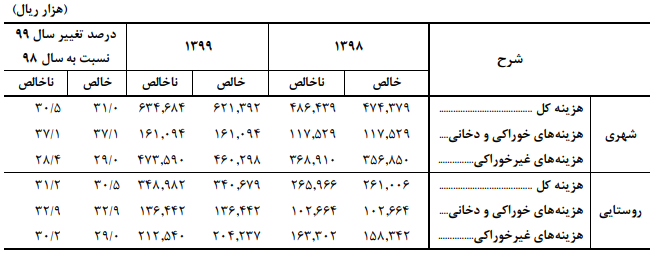
\includegraphics[scale=0.8]{costs.png}
%	\caption{متوسط هزینه‌ی کل، خوراکی و دخانی و غیرخوراکی خالص و ناخالص سالانه‌ی یک خانوار شهری و روستایی سال 1398 و 1399 \\
%	منبع: چکیده‌ی نتایج طرح آمارگیری هزینه و درآمد خانوارهای شهری و روستایی سال 1399}
%\label{costs}
%\end{figure}}



\section{Model}
We use the DLLM method to estimate poverty dynamics, which based on  a consumption model is constructed for each  year of 1 and  2:

\begin{align}
	C_{i1} = \beta'_1X_{i1} + \epsilon_{i1}
	\label{eq1}
\end{align}
\begin{align}
	C_{j2} = \beta'_2X_{j2} + \epsilon_{j2}
	\label{eq2}
\end{align}
Where, C is the variable of consumption, i and j represents the households, $X_i$ is the vector of time-invariant covariates, $\beta$ is the vector of parameters to be estimated, and $\epsilon$ is the error term. The consumption of year 1 for household j who is surveyed in year 2 is not observable, but it can be estimated. The two equations are estimated using Ordinary Least Squares (OLS) regression.
The variables selected for the models are: Household’s head age, sex, number of years of education, number of children, area of living (urban/rural), province, household’s size, status of employment (employed/unemployed) and status of marriage (married/single) of the household's head.

The DLLM method makes two key assumptions: first, that the underlying population sampled is the same in both years, and second, that the error terms are positive quadrant dependent, which implies that the correlation of the error terms is non-negative. Based on these assumptions, we can derive nonparametric bounds. The upper bound estimates are given by the probability that the two error terms are completely independent of each other. To derive the nonparametric upper bounds, for each household j in round 2, a random draw with replacement is taken from the empirical distribution of the predicted residuals and the consumption of year 1 is estimated using the following equation:
	 
	 \begin{align*}
	 	\widehat{C_{j1}^U} = \hat{\beta}'_1X_{j2} + \check{\epsilon_{j1}}
	 \end{align*}
 % که 
 % $\check{\epsilon_{j1}}$
 % جمله‌ی باقیمانده‌ای است که در هر $j$ جایگذاری شده است. اکنون داده‌ی تابلویی ساختگی ساخته شده است که می‌توانیم به کمک آن پویایی فقر را محاسبه کنیم.
 
 The lower bound estimates are given by the probability that 
 the two error terms in the consumption model are completely dependent on each other. the consumption of year 1 is estimated using the following equation:
 
 \begin{align*}
 	\widehat{C_{j1}^L} = \hat{\beta}'_1X_{j2} + \gamma \hat{\epsilon}_{j2}
 \end{align*}
 Where scalar $\gamma$ is chosen to ensure the standard deviation of the imputed Year 1 residuals distribution equals $\hat{\sigma}_1$. 

In order to narrow the bounds, \citet{dang2014using} propose a parametric approach that assumes that the two consumption-model errors have a bivariate normal distribution. Let $\rho=\operatorname{Corr}(\epsilon_{j1},\epsilon_{j2})$ denote the intertemporal correlation between the unexplained components of consumption for the same household, conditional on the observed covariates. Thus, $\rho$ measures persistence in unobserved household circumstances and shocks; it is not the correlation between observed consumption levels. Under this specification, the probability that household $j$ is poor in both periods is
\begin{align}
	\Pr(C_{j1}<z_1,\ C_{j2}<z_2) = \Phi_2 \left(\dfrac{z_1-\beta'_1X_{j2}}{\sigma_1}, \dfrac{z_2-\beta'_2X_{j2}}{\sigma_2};\rho \right)
	\label{eq:joint-poor}
\end{align}

Independent repeated cross-sections identify the two marginal residual distributions, but they do not observe $\epsilon_{j1}$ and $\epsilon_{j2}$ jointly for the same household. Consequently, $\rho$ is not point-identified from the repeated cross-sections alone. A lower value of $\rho$ implies less persistence in unobserved welfare and therefore more estimated entry into and exit from poverty. A higher value implies greater persistence, increasing the poor--poor and nonpoor--nonpoor probabilities while reducing the two transition probabilities. In the DLLM terminology, the higher endpoint $\rho_H$ produces the lower bound on mobility and the upper bound on immobility, whereas the lower endpoint $\rho_S$ produces the upper bound on mobility and the lower bound on immobility \citep[pp.~113--120]{dang2014using}.

We therefore report results over alternative plausible intervals for $\rho$ rather than imposing a single value. Specification~1 uses the full non-negative interval $[0,1]$. The panel estimates reported by \citet{dang2014using} for six developing countries range from 0.39 to 0.66; to allow for cross-country and model uncertainty, the authors evaluate the wider intervals $[0.2,0.8]$ and $[0.3,0.7]$, which form Specifications~2 and~3 in this study. These intervals are sensitivity assumptions, not estimates from the Iranian repeated cross-sections. Narrower intervals produce tighter bounds, but the additional precision depends on stronger external restrictions and carries a greater risk of excluding the true transition rate \citep[pp.~119--121]{dang2014using}.

% \subsection{Poverty Line: The \$6.85 per Day (2017 PPP) Threshold}
% The \$6.85 per day threshold, measured in 2017 Purchasing Power Parity (PPP), is a standardized international poverty line established by the World Bank for assessing poverty in upper-middle-income countries \citep{WorldBank2020}. It is derived from the International Comparison Program's (ICP) 2017 benchmark, which provides conversion factors that equalize purchasing power across currencies, enabling meaningful cross-country comparisons by accounting for differences in national price levels \citep{WorldBank2017}. This line is part of a tiered measurement system that also includes an extreme poverty line (\$2.15) and a lower-middle-income line (\$3.65), allowing for nuanced analysis of economic well-being across different development contexts \citep{Jolliffe2022}.

% The use of the 2017 PPP update, including the \$6.85 line, is methodologically justified for several reasons. First, it maintains \emph{temporal comparability}: PPPs are not static, and the 2017 benchmark incorporates more recent price data, reducing biases inherent in outdated conversion factors \citep{Deaton2010}. Second, it ensures \emph{cross-country consistency}, creating a standardized welfare metric that allows for coherent global poverty aggregation and comparison, which is essential for tracking progress toward international targets like Sustainable Development Goal 1 \citep{Ravallion2016}. Third, it addresses a measurement gap in \emph{higher development contexts}, where the extreme poverty line becomes less informative; the \$6.85 threshold better captures economic vulnerability and modest living standards prevalent in upper-middle-income countries \citep{Ferreira2016}. Finally, it aligns with the \emph{evolving global income distribution}, facilitating the study of poverty gradations and enabling a more comprehensive assessment of inclusive growth \citep{Lakner2020}.

% Nonetheless, PPP-based measures have recognized limitations. The construction of PPPs is methodologically complex, and revisions can create discontinuities in historical poverty series \citep{Deaton2005}. Critics also note that uniform international lines may not adequately reflect locally specific needs and social definitions of poverty \citep{Reddy2008}. Consequently, best practice recommends that the \$6.85 (2017 PPP) line be used \emph{in conjunction with} national poverty lines and complementary multidimensional deprivation indices \citep{Alkire2011}.

\subsection{Poverty Line: The \$8.30 per Day (2021 PPP) Threshold}
As global living standards have risen, so too have the methods for measuring poverty. Successive revisions to the international poverty line—implemented in 2001, 2008, 2015, 2022, and most recently this month—reflect improvements in consumption measurement, updates to national poverty thresholds, and the use of Purchasing Power Parities (PPPs) to harmonize costs and incomes across countries. The current update, which also affects middle-income country lines, draws on new PPPs from the 2021 International Comparison Program and incorporates recent changes in national poverty benchmarks—a key factor behind the notable rise in the extreme poverty threshold.
Based on these revised factors, the international poverty line for low-income countries is now up from \$2.15 \text{ to} \$3 per person per day. For lower middle-income countries it’s changed from \$3.65 \text{ to} \$4.15 per day and for upper middle-income countries it went up from \$6.85 \text{ to} \$8.30. 

The \$8.30 per day threshold, measured in 2021 Purchasing Power Parity (PPP), now is a standardized international poverty line established by the World Bank for assessing poverty in upper-middle-income countries \citep{Foster2025GlobalPoverty,WorldBank2025GlobalPovertyLines}. It is derived from national poverty lines expressed in 2021 PPP dollars; the median among upper-middle-income countries is \$8.29 and is rounded to \$8.30 \citep[Section~3.1 and Table~1]{Foster2025GlobalPoverty}. This line is part of a tiered measurement system that also includes an extreme poverty line (\$3.00) and a lower-middle-income line (\$4.15), allowing for a more nuanced analysis of economic well-being across development contexts \citep{Foster2025GlobalPoverty,WorldBank2025GlobalPovertyLines}.

The use of the 2021 PPP update, including the \$8.30 line, is methodologically justified for several reasons. First, it uses a \emph{current price benchmark}: the 2021 PPPs incorporate more recent price data, while the revised poverty lines draw on updated national poverty lines \citep{Foster2025GlobalPoverty}. Second, it ensures \emph{cross-country consistency}, creating a standardized welfare metric that allows for coherent global poverty aggregation and comparison \citep{Foster2025GlobalPoverty}. Third, it addresses a measurement gap in \emph{higher development contexts}, where the extreme poverty line is less informative; the \$8.30 threshold provides a more relevant benchmark for upper-middle-income countries \citep{WorldBank2025GlobalPovertyLines}. Finally, it aligns the analysis with the World Bank's current global poverty reporting framework, while the corresponding 2017 PPP series remains available through the Poverty and Inequality Platform \citep{WorldBank2025GlobalPovertyLines}.

Nonetheless, PPP-based measures have recognized limitations. The construction of PPPs is methodologically complex, and revisions can alter measured poverty levels and create discontinuities in historical poverty series \citep{Deaton2010,Foster2025GlobalPoverty}. Uniform international lines may also fail to reflect locally specific needs and national definitions of poverty; national poverty lines are therefore more appropriate for country-specific policy dialogue and targeting \citep{WorldBank2025GlobalPovertyLines}. Consequently, the \$8.30 (2021 PPP) line is used in this study as an international benchmark and should be considered alongside national poverty lines and, where relevant, complementary multidimensional deprivation measures \citep{WorldBank2025GlobalPovertyLines,Alkire2011}.


%
%در یک بررسی اولیه، حدود ناپارامتریک برای سال‌های 1398 و 1399 محاسبه شده و نتایج آن در جدول \ref{table1} قابل مشاهده است. برای محاسبه‌ی این حدود، تنها یک مدل در ساده‌ترین شکل آن و با متغیرهای مستقل سن، جنسیت و سال‌های تحصیل سرپرست تخمین زده شده است. خط فقر سال‌های 1398 و 1399 بر مبنای روش ارائه‌شده توسط 
%\cite{majlis1395poverty}
%محاسبه‌ شده است که به‌ترتیب برابر با 8,248,972 ریال و 10,857,318 ریال سرانه در ماه است. ستون 
%\lr{Truth}
%نشان می‌دهد که مقدار واقعی پویایی برای خانوارهای مشترک در این دو سال به چه میزان بوده است. به‌عنوان مثال، بر اساس نتیجه‌ی به‌دست آمده، بین ۲٫۳ تا 16٫۷درصد از جمعیت کشور در این دو سال از فقر خارج شده‌اند. مشاهده می‌شود که در تمام حالات حدود ناپارامتریک دربردارنده‌ی مقدار واقعی پویایی است؛ اگرچه به‌دلیل سادگی مدل و استفاده از روش ناپارامتریک حد بالا و حد پایین فاصله‌ی قابل‌توجهی با یکدیگر دارند که این مسئله اهمیت تعریف دقیق مدل و استفاده از روش پارامتریک را نشان می‌دهد.
%
%\begin{table}[h!]
%	\captionsetup{font=scriptsize}
%%	\captionsetup{justification=centering}
%%	 \captionsetup{labelsep=newline}
%	\begin{latin}
%	\centering
%	\begin{tabular}{lllr}
%		\toprule \toprule
%		1398-1399	&         Lower Bound  & Truth & Upper Bound       \\
%		\midrule
%		Poor, poor              &  27.99    & 23.08 & 11.46             \\
%		& & (0.3) & \\
%		Poor,nonpoor                &      0   & 9.7 &29.19     \\
%		& & (0.2) & \\
%		&                     \\
%		[1em]
%		Nonpoor, poor            &       0.19     & 10 & 16.70     \\
%		& & (0.2) & \\
%		&                     \\
%		[1em]
%		Nonpoor, nonpoor               &      71.83   & 57 & 42.63      \\
%		& & (0.3) & \\
%		\bottomrule\bottomrule
%	\end{tabular}
%\end{latin}
%\caption[]{درصد پویایی فقر، محاسبه‌شده با استفاده از داده‌های طرح هزینه و درآمد خانوار سال‌های 1398 و 1399\newline
%اعداد داخل پرانتز خطای معیار را نشان می‌دهند}
%\label{table1}
%\end{table}

\section{Results}
The present study examines poverty dynamics in two consequent years of 2019 and 2020, with a secondary objective of validating the results of the synthetic panel approach against those of true panel data. Table \autoref{tab:table1} presents the results for all urban and rural households. Three specifications are considered, with varying assumptions on the correlation between error terms ($\rho$).
Specification 1 uses $\rho_H=1$ for the lower bounds and $\rho_S=0$ for the upper bounds, representing the parametric analogue of the nonparametric bounds. Specification 2 uses $\rho_H=0.8$ and $\rho_S=0.2$ as the higher and lower endpoints, respectively. Specification 3 further narrows the bounds by using $\rho_H=0.7$ and $\rho_S=0.3$. It is expected that each specification provides narrower bounds compared to the previous specification, however, this also increases the possibility that the true poverty dynamic rates from the panel data fall outside of the bounds.



The synthetic panel approach performs well in replicating true poverty dynamics, as shown in Table \autoref{tab:table1}. The genuine panel rates consistently fall within the estimated lower and upper bounds across all specifications. Under the parametric Specification 3, for example, the true persistence rate—households poor in both 2019 and 2020—lies between 8.8\% and 11.8\%. This finding is statistically proved by the nonparametric bound that ranges from 6.7\% to 14.6\%, this fraction of households are suffering from chronic poverty. Across all transition categories, the true rates fall within the estimated bounds, confirming the validity of the synthetic approach. The true panel data indicate that 9.4\% of households remained poor in both periods (chronic poverty), 7.5\% escaped poverty, and 9.9\% fell into poverty—the highest transition rate, reflecting substantial downward mobility likely driven by macroeconomic volatility, high inflation, and sanctions. These findings underscore the importance of distinguishing between chronic and transitory poverty and highlight the vulnerability of non-poor households, particularly within the shrinking middle class.

	
	\begin{table}[H]
    \scriptsize
    \centering
    \caption{Poverty dynamics for all rural and urban households}
    \label{tab:table1}
       \begin{tabular}{lccccccccc}
        \toprule
        Poverty Status
        & \multicolumn{1}{c}{\shortstack{Nonparametric\\bound}}
        & \multicolumn{3}{c}{Parametric lower bound}
        & \multicolumn{1}{c}{Truth}
        & \multicolumn{3}{c}{Parametric upper bound}
        & \multicolumn{1}{c}{\shortstack{Nonparametric\\bound}} \\
        \cmidrule(lr){3-5} \cmidrule(lr){7-9}
        & & Spec. 1 & Spec. 2 & Spec. 3 & & Spec. 3 & Spec. 2 & Spec. 1 & \\
        \midrule

        Poor, poor
        & 14.6 & 16.1 & 12.9 & 11.8 & 9.4 & 8.8 & 8.2 & 7.1 & 6.7 \\
        Std. Dev.
        &     &     &     &     & 0.4 &     &     &     &     \\
        \addlinespace[0.2em]

        Poor, nonpoor
        & 1.1 & 0.9 & 4.1 & 5.1 & 7.5 & 8.1 & 8.7 & 9.9 & 9.8 \\
        Std. Dev.
        &     &     &     &     & 0.5 &     &     &     &     \\
        \addlinespace[0.2em]

        Nonpoor, poor
        & 3.4 & 3.3 & 6.5 & 7.5 & 9.9 & 10.6 & 11.2 & 12.3 & 11.2 \\
        Std. Dev.
        &     &     &     &     & 0.5 &     &     &     &     \\
        \addlinespace[0.2em]

        Nonpoor, nonpoor
        & 80.9 & 79.7 & 76.6 & 75.5 & 73.1 & 72.5 & 71.9 & 70.8 & 72.3 \\
        Std. Dev.
        &      &      &      &      & 0.6 &      &      &      &      \\
        \midrule

        N
        & 5799 & 5799 & 5799 & 5799 & 11485 & 5799 & 5799 & 5799 & 5799 \\
        \bottomrule
    \end{tabular}
    \caption*{ \footnotesize \textbf{Note:}  This table presents poverty dynamics between two consecutive years, 2019 and 2020. The HIES data come from a rotating survey that tracks three-quarters of households in subsequent waves. The "Truth" column reports poverty status calculated from the genuine panel, while Specifications 1–3 apply the DLLM synthetic methodology to estimate lower and upper bounds. Across all specifications, the estimated bounds consistently contain the true poverty transition rates.  1. Poverty rates in percent are calculated using HIES data, statistical Center of Iran, and predictions obtained using data in the second survey rounds.
Full regression results are provided in Tables 2.1a and 2.1b in Appendix ??. \\
2. All calculations are weighted using population weights for each survey round. Standard errors in parentheses.\\
3. Number of replications for the estimates is 500.\\
4. Household heads' ages are restricted to between 25 and 55 in the first survey round.}
\end{table}
To further explore poverty dynamics in Iran, we extend the analysis to specific population subgroups. Table \autoref{tab:table2} focuses on female-headed households. The estimates indicate that these households face a higher probability of persistent poverty relative to other household types. This result is consistent with the established finding that women encounter greater poverty risk due to restricted labor market participation and occupational segregation. Female-headed households often bear disproportionate caregiving burdens and, lacking access to remunerative employment, frequently depend on informal, part-time, or low-wage work \citep{yoosefi2020challenges}. These findings underscore the necessity of incorporating gender-sensitive approaches into poverty reduction policies.


\begin{table}[H]
    \scriptsize
    \centering
    \caption{Poverty dynamics for female-headed households}
    \label{tab:table2}
        \begin{tabular}{lccccccccc}
    \toprule
    Poverty Status
    & \multicolumn{1}{c}{\shortstack{Nonparametric\\bound}}
    & \multicolumn{3}{c}{Parametric lower bound}
    & \multicolumn{1}{c}{Truth}
    & \multicolumn{3}{c}{Parametric upper bound}
    & \multicolumn{1}{c}{\shortstack{Nonparametric\\bound}} \\
    \cmidrule(lr){3-5} \cmidrule(lr){7-9}
    & & Spec. 1 & Spec. 2 & Spec. 3 & & Spec. 3 & Spec. 2 & Spec. 1 & \\
    \midrule

    Poor, poor
    & 18.8 & 21.5 & 18.6 & 17.5 & 14.8 & 14.0 & 13.3 & 11.9 & 12.4 \\
    Std. Dev.
    &      &      &      &      & 1.7  &      &      &      &      \\
    \addlinespace[0.2em]

    Poor, nonpoor
    & 3.8 & 2.7 & 5.6 & 6.7 & 9.4 & 10.2 & 10.9 & 12.3 & 11.5 \\
    Std. Dev.
    &     &     &     &     & 1.9 &     &     &     &     \\
    \addlinespace[0.2em]

    Nonpoor, poor
    & 7.8 & 5.1 & 8.0 & 9.1 & 11.9 & 12.6 & 13.3 & 14.7 & 14.2 \\
    Std. Dev.
    &     &     &     &     & 1.9 &     &     &     &     \\
    \addlinespace[0.2em]

    Nonpoor, nonpoor
    & 69.6 & 70.7 & 67.8 & 66.7 & 63.9 & 63.2 & 62.5 & 61.1 & 61.9 \\
    Std. Dev.
    &      &      &      &      & 2.6  &      &      &      &      \\
    \midrule

    N
    & 441 & 441 & 441 & 441 & 862 & 441 & 441 & 441 & 441 \\
    \bottomrule
\end{tabular}
    \caption*{ \footnotesize \textbf{Note:}   1. Poverty rates in percent are calculated using HIES data, statistical Center of Iran, and predictions obtained using data in the second survey rounds.
Full regression results are provided in Tables 2.1a and 2.1b in Appendix ??. \\
2. All calculations are weighted using population weights for each survey round. Standard errors in parentheses.\\
3. Number of replications for the estimates is 500.\\
4. Household heads' ages are restricted to between 25 and 55 in the first survey round. }
\end{table}

Table \autoref{tab:table2} presents poverty transition rates for female-headed households between 2019 and 2020. The true panel data reveal that 14.8\% of female-headed households remained poor in both periods-substantially higher than the 9.4\% rate observed for all households. This substantially higher chronic poverty rate reflects the structural barriers women face in accessing stable, well-paid employment \citep{yoosefi2020challenges}. Additionally, 11.9\% of female-headed households fell into poverty during this period (compared to 9.9\% overall), while only 63.9\% remained non-poor in both years (versus 73.1\% overall). These findings highlight the heightened vulnerability of female-headed households to poverty and underscore the need for gender-responsive poverty reduction policies that address both chronic deprivation and the risk of future impoverishment.

Education influences chronic poverty primarily through its effect on labor market opportunities and earning capacity.  Higher educational attainment is widely recognized as a pathway to improved employability and greater income-earning potential \citep{bilenkisi2015impact}. Table \ref{table3} reports poverty transition rates for households headed by individuals without a university degree. The results show that these households face a higher probability of persistent poverty than those with university-educated heads. These findings reinforce the critical role of investment in education and skill development in reducing poverty and fostering upward economic mobility.

\begin{table}[H]
    \scriptsize
    \centering
    \caption{Poverty dynamics among households with non-university-educated heads}
    \label{tab:table3}
\begin{tabular}{lccccccccc}
    \toprule
    Poverty Status
    & \multicolumn{1}{c}{\shortstack{Nonparametric\\bound}}
    & \multicolumn{3}{c}{Parametric lower bound}
    & \multicolumn{1}{c}{Truth}
    & \multicolumn{3}{c}{Parametric upper bound}
    & \multicolumn{1}{c}{\shortstack{Nonparametric\\bound}} \\
    \cmidrule(lr){3-5} \cmidrule(lr){7-9}
    & & Spec. 1 & Spec. 2 & Spec. 3 & & Spec. 3 & Spec. 2 & Spec. 1 & \\
    \midrule

    Poor, poor
    & 17.7 & 19.1 & 15.1 & 13.9 & 11.0 & 10.4 & 9.7 & 8.3 & 8.0 \\
    Std. Dev.
    &      &      &      &      & 0.5 &      &      &      &      \\
    \addlinespace[0.2em]

    Poor, nonpoor
    & 0.9 & 0.8 & 4.7 & 5.9 & 8.8 & 9.5 & 10.2 & 11.5 & 11.3 \\
    Std. Dev.
    &     &     &     &     & 0.5 &     &     &     &     \\
    \addlinespace[0.2em]

    Nonpoor, poor
    & 2.4 & 3.1 & 7.1 & 8.3 & 11.1 & 11.8 & 12.5 & 13.8 & 12.2 \\
    Std. Dev.
    &     &     &     &     & 0.5 &     &     &     &     \\
    \addlinespace[0.2em]

    Nonpoor, nonpoor
    & 78.9 & 77.0 & 73.1 & 71.9 & 69.1 & 68.3 & 67.6 & 66.3 & 68.6 \\
    Std. Dev.
    &      &      &      &      & 0.8 &      &      &      &      \\
    \midrule

    N
    & 5172 & 5172 & 5172 & 5172 & 10201 & 5172 & 5172 & 5172 & 5172 \\
    \bottomrule
\end{tabular}


     \caption*{ \footnotesize \textbf{Note:}   1. Poverty rates in percent are calculated using HIES data, statistical Center of Iran, and predictions obtained using data in the second survey rounds.
Full regression results are provided in Tables 2.1a and 2.1b in Appendix ??. \\
2. All calculations are weighted using population weights for each survey round. Standard errors in parentheses.\\
3. Number of replications for the estimates is 500.\\
4. Household heads' ages are restricted to between 25 and 55 in the first survey round.}
\end{table}


\begin{table}[H]
    \scriptsize
    \centering
    \caption{Poverty dynamics for households with a university-educated head}
    \label{tab:table3_2}
    \begin{tabular}{lccccccccc}
    \toprule
    Poverty Status
    & \multicolumn{1}{c}{\shortstack{Nonparametric\\bound}}
    & \multicolumn{3}{c}{Parametric lower bound}
    & \multicolumn{1}{c}{Truth}
    & \multicolumn{3}{c}{Parametric upper bound}
    & \multicolumn{1}{c}{\shortstack{Nonparametric\\bound}} \\
    \cmidrule(lr){3-5} \cmidrule(lr){7-9}
    & & Spec. 1 & Spec. 2 & Spec. 3 & & Spec. 3 & Spec. 2 & Spec. 1 & \\
    \midrule

    Poor, poor
    & 1.9 & 2.4 & 1.7 & 1.5 & 0.9 & 0.7 & 0.6 & 0.4 & 0.3 \\
    Std. Dev.
    &      &      &      &      & 0.4 &      &      &      &      \\
    \addlinespace[0.2em]

    Poor, nonpoor
    & 0.0 & 0.1 & 0.8 & 1.0 & 1.6 & 1.8 & 1.9 & 2.1 & 1.8 \\
    Std. Dev.
    &     &     &     &     & 0.6 &     &     &     &     \\
    \addlinespace[0.2em]

    Nonpoor, poor
    & 2.5 & 2.8 & 3.5 & 3.7 & 4.3 & 4.5 & 4.6 & 4.8 & 4.1 \\
    Std. Dev.
    &     &     &     &     & 0.9 &     &     &     &     \\
    \addlinespace[0.2em]

    Nonpoor, nonpoor
    & 95.6 & 94.7 & 94.1 & 93.8 & 93.2 & 93.0 & 92.9 & 92.7 & 93.8 \\
    Std. Dev.
    &      &      &      &      & 1.1 &      &      &      &      \\
    \midrule

    N
    & 664 & 664 & 664 & 664 & 1309 & 664 & 664 & 664 & 664 \\
    \bottomrule
\end{tabular}

     \caption*{ \footnotesize \textbf{Note:}  This table illustrates that between 2019 and  2020.  1. Poverty rates in percent are calculated using HIES data, statistical Center of Iran, and predictions obtained using data in the second survey rounds.
Full regression results are provided in Tables 2.1a and 2.1b in Appendix ??. \\
2. All calculations are weighted using population weights for each survey round. Standard errors in parentheses.\\
3. Number of replications for the estimates is 500.\\
4. Specification 1 uses $\rho_H=1$ and $\rho_S=0$ for the lower and upper bounds, respectively, and is the parametric analogue of the nonparametric bounds. Specification 2
uses $\rho_H=0.8$ and $\rho_S=0.2$, and Specification 3 uses $\rho_H=0.7$ and $\rho_S=0.3$ for the lower and upper bounds, respectively. The regressors in all regressions are the
same as in Model 1 in Table 1 plus an urban/rural dummy variable.
5. Household heads' ages are restricted to between 25 and 55 in the first survey round.}
\end{table}
The protective effect of education against chronic poverty is strikingly  evident when comparing households by the head's educational attainment. Among households with non-university-educated heads (Table \autoref{tab:table3}), 11.0\% remained poor in both periods, and 11.1\% fell into poverty between 2019 and 2020—rates significantly higher than the full-sample averages of 9.4\% and 9.9\%, respectively. By contrast, households with university-educated heads (Table \ref{table3_2}) exhibit substantially lower poverty persistence (0.9\%) and entry rates (4.3\%), with 93.2\% maintaining nonpoor status across both periods. These findings confirm that higher education serves as a critical safeguard against poverty, enhancing employability and income-earning potential while reducing vulnerability to economic shocks \citep{bilenkisi2015impact}. The education gap in poverty outcomes—a 10.1 percentage point difference in chronic poverty and a 24.1 percentage point gap in sustained non-poverty—underscores the importance of investment in education and skills training as a strategy for poverty reduction and economic mobility.

%\begin{table}[H]
%	\small
%	\tabcolsep=0.11cm
%	\noindent\makebox[\textwidth]{
%		\begin{tabular}{rccccccccc}
%			وضعیت فقر               & حد ناپارامتریک       & \multicolumn{3}{c}{حد بالا - پارامتریک}                            & مقدار واقعی          & \multicolumn{3}{c}{حد پایین - پارامتریک}                           & حد ناپارامتریک       \\ \cline{3-5} \cline{7-9}
%			&                      & حالت ۱               & حالت ۲               & حالت ۳               &                      & حالت ۳               & حالت ۲               & حالت ۱               &                      \\ \hline
%			Poor, poor       & $3/4$                 & $4/1                 $& $5/2$                 & $5/8$                 & $5/2                   $& $8/8$                 & $9/8$                 & $12/4                 $& $10/6$                 \\
%			Standard Deviation         &                      &                      &                      &                      & $0/6                  $&                      &                      &                      &                      \\
%			Poor, nonpoor    & $8/2$                  & $8/6$& $7/5$                  & $6/8$                    & $3                 $& $3/8$                 & $2/8$                 & $0/3                 $& $0/1$                 \\
%			Standard Deviation         &                      &                      &                      &                      & $0/5                  $&                      &                      &                      &                      \\
%			Nonpoor, poor   & $11/4$                  & $15/4$& $14/3$                  & $13/7$                 & $9/3                 $& $10/7$                 & $9/7$                 & $7/1                 $& $4/1$                 \\
%			Standard Deviation         &                      &                      &                      &                      & $0/8                  $&                      &                      &                      &                      \\
%			Nonpoor, nonpoor & $77/1$                 & $71/9$& $73$                 & $73/7$                 & $82/5                 $& $76/7$                 & $77/7$                 & $80/2                 $& $85/1$                 \\
%			Standard Deviation         &                      &                      &                      &                      & $1/1                  $&                      &                      &                      &                      \\
%			\multicolumn{1}{l}{}    & \multicolumn{1}{l}{} & \multicolumn{1}{l}{} & \multicolumn{1}{l}{} & \multicolumn{1}{l}{} & \multicolumn{1}{l}{} & \multicolumn{1}{l}{} & \multicolumn{1}{l}{} & \multicolumn{1}{l}{} & \multicolumn{1}{l}{} \\\hline
%			N           &651                 & 651& 651& 651& 1296& 651                 & 651                 & 651                 & 651                
%	\end{tabular}}
%	\caption{تخمین پویایی فقر برای خانوارهایی که سرپرست دارای تحصیلات دانشگاهی است.}
%	\label{haveduc}
%\end{table}

Tables \autoref{table4} and \autoref{table5} present the poverty dynamics of urban and rural households separately. The results show that the probability of remaining in poverty is higher for rural households as compared to urban households. Additionally, the rate of poverty transition (moving into or out of poverty in 2020) is lower for urban households as compared to rural households. These findings suggest that rural households are disproportionately affected by poverty and may require targeted interventions to reduce poverty and improve economic mobility. The higher poverty transition rate and lower probability of remaining in poverty for urban households may be due to the greater economic opportunities and access to services in urban areas. Overall, these findings highlight the importance of considering the specific needs and challenges faced by rural households in poverty reduction policies and programs.



\begin{table}[H]
    \scriptsize
    \centering
    \caption{Poverty dynamics of urban households.}
    \label{table4}
 \begin{tabular}{lccccccccc}
    \toprule
    Poverty Status
    & \multicolumn{1}{c}{\shortstack{Nonparametric\\bound}}
    & \multicolumn{3}{c}{Parametric lower bound}
    & \multicolumn{1}{c}{Truth}
    & \multicolumn{3}{c}{Parametric upper bound}
    & \multicolumn{1}{c}{\shortstack{Nonparametric\\bound}} \\
    \cmidrule(lr){3-5} \cmidrule(lr){7-9}
    & & Spec. 1 & Spec. 2 & Spec. 3 & & Spec. 3 & Spec. 2 & Spec. 1 & \\
    \midrule

    Poor, poor
    & 8.2 & 10.3 & 7.8 & 7.1 & 5.3 & 4.8 & 4.3 & 3.5 & 2.8 \\
    Std. Dev.
    &      &      &      &      & 0.5 &      &      &      &      \\
    \addlinespace[0.2em]

    Poor, nonpoor
    & 0.8 & 0.7 & 3.1 & 3.9 & 5.6 & 6.2 & 6.7 & 7.5 & 7.8 \\
    Std. Dev.
    &     &     &     &     & 0.5 &     &     &     &     \\
    \addlinespace[0.2em]

    Nonpoor, poor
    & 2.7 & 2.8 & 5.3 & 6.1 & 7.8 & 8.4 & 8.8 & 9.6 & 8.1 \\
    Std. Dev.
    &     &     &     &     & 0.6 &     &     &     &     \\
    \addlinespace[0.2em]

    Nonpoor, nonpoor
    & 88.3 & 86.2 & 83.7 & 82.9 & 81.3 & 80.6 & 80.2 & 79.4 & 81.3 \\
    Std. Dev.
    &      &      &      &      & 0.8 &      &      &      &      \\
    \midrule

    N
    & 2987 & 2987 & 2987 & 2987 & 5873 & 2987 & 2987 & 2987 & 2987 \\
    \bottomrule
\end{tabular}

    
    \vspace{0.5em} 
    \begin{minipage}{\linewidth} 
    \caption*{\scriptsize \textbf{Note:}This table illustrates that between 2019 and  2020.  1. Poverty rates in percent are calculated using HIES data, statistical Center of Iran, and predictions obtained using data in the second survey rounds.
Full regression results are provided in Tables 2.1a and 2.1b in Appendix ??. \\
2. All calculations are weighted using population weights for each survey round. Standard errors in parentheses.\\
3. Number of replications for the estimates is 500.\\
4. Specification 1 uses $\rho_H=1$ and $\rho_S=0$ for the lower and upper bounds, respectively, and is the parametric analogue of the nonparametric bounds. Specification 2
uses $\rho_H=0.8$ and $\rho_S=0.2$, and Specification 3 uses $\rho_H=0.7$ and $\rho_S=0.3$ for the lower and upper bounds, respectively. The regressors in all regressions are the
same as in Model 1 in Table 1 plus an urban/rural dummy variable.
5. Household heads' ages are restricted to between 25 and 55 in the first survey round.} 
    \end{minipage}
\end{table}

\begin{table}[H]
    \scriptsize
    \centering
    \caption{Poverty dynamics of rural households.}
    \label{table5}
  \begin{tabular}{lccccccccc}
    \toprule
    Poverty Status
    & \multicolumn{1}{c}{\shortstack{Nonparametric\\bound}}
    & \multicolumn{3}{c}{Parametric lower bound}
    & \multicolumn{1}{c}{Truth}
    & \multicolumn{3}{c}{Parametric upper bound}
    & \multicolumn{1}{c}{\shortstack{Nonparametric\\bound}} \\
    \cmidrule(lr){3-5} \cmidrule(lr){7-9}
    & & Spec. 1 & Spec. 2 & Spec. 3 & & Spec. 3 & Spec. 2 & Spec. 1 & \\
    \midrule

    Poor, poor
    & 32.9 & 33.4 & 28.3 & 26.7 & 22.1 & 21.6 & 20.6 & 18.6 & 18.5 \\
    Std. Dev.
    &      &      &      &      & 0.8 &      &      &      &      \\
    \addlinespace[0.2em]

    Poor, nonpoor
    & 0.6 & 1.0 & 6.1 & 7.7 & 12.1 & 12.7 & 13.8 & 15.8 & 15.8 \\
    Std. Dev.
    &     &     &     &     & 0.7 &     &     &     &     \\
    \addlinespace[0.2em]

    Nonpoor, poor
    & 5.4 & 5.4 & 10.5 & 12.1 & 16.7 & 17.1 & 18.2 & 20.2 & 19.8 \\
    Std. Dev.
    &     &     &     &     & 0.9 &     &     &     &     \\
    \addlinespace[0.2em]

    Nonpoor, nonpoor
    & 61.1 & 60.3 & 55.2 & 53.5 & 49.1 & 48.5 & 47.5 & 45.5 & 45.9 \\
    Std. Dev.
    &      &      &      &      & 1.0 &      &      &      &      \\
    \midrule

    N
    & 2865 & 2865 & 2865 & 2865 & 5627 & 2865 & 2865 & 2865 & 2865 \\
    \bottomrule
\end{tabular}

    \caption*{\scriptsize \textbf{Note:} This table illustrates that between 2019 and  2020....}  
\end{table}

\section{Robustness Checks} 
To evaluate the robustness of our findings, we extend the analysis to cover multiple transition windows: 2020-2021, 2021-2022, 2022-2023, and 2023-2024. We also examine in this section robustness to the choice of subpopulation groups. This multi-period approach is essential in the Iranian context, where the economy has been characterized by sustained inflationary pressures and recurrent sanctions-induced shocks \citep{WorldBank2023, EslamiHoseini2024}. In such a highly volatile setting, single-period poverty transition estimates may be influenced by short-term fluctuations rather than reflecting enduring structural patterns \citep{BaulchHoddinott2000}. By replicating the analysis across several consecutive years, we can ascertain whether the observed poverty dynamics—particularly the heightened chronic poverty among female-headed and less-educated households—remain consistent over time or are specific to particular economic episodes \citep{BarrettCarter2016}. This robustness strategy strengthens the reliability of our inferences and offers a more detailed picture of poverty persistence and vulnerability in Iran's unstable economic environment \citep{Ravallion2001, Dercon2005}.
\subsection{Robustness of Findings Across Time}

To assess the robustness of our findings, we extended the analysis to cover four consecutive transition periods: 2020-2021, 2021-2022, 2022-2023, and 2023-2024, which are reported in  \autoref{tab:all_99_1400}  to  \autoref{tab:rural_1402_1403}. This multi-period approach is particularly important in the Iranian context, where the economy has been subjected to persistent inflationary pressures and recurring sanctions-induced shocks. In such a volatile environment, poverty dynamics observed in a single year may reflect transitory fluctuations rather than enduring structural patterns. By examining poverty transitions across several consecutive periods, we can determine whether the observed relationships—such as the elevated chronic poverty among female-headed and non-college-educated households—are stable over time or merely artifacts of specific economic episodes.

The results consistently confirm our main findings across all periods. For the full sample, chronic poverty rates (Poor to Poor) range from 6.0\% to 11.0\% across the four periods, with the highest rate observed in 2020-2021 (11.0\%) and the lowest in 2023-2024 (6.0\%). This declining trend in chronic poverty is accompanied by a corresponding increase in sustained non-poverty (Nonpoor to Nonpoor), which rises from 69.2\% in 2020-2021 to 81.0\% in 2023-2024, suggesting a gradual improvement in household welfare over the period-potentially reflecting the recovery from the immediate shocks of the early 2020s. However, poverty entry rates (Nonpoor to Poor) remain substantial, ranging from 6.0\% to 11.1\%, indicating that vulnerability to poverty persists despite overall improvements.

The subgroup analyses reinforce the robustness of our key findings. Female-headed households consistently exhibit the highest chronic poverty rates across all periods, ranging from 8.6\% in 2023-2024 to 15.5\% in 2020-2021, substantially exceeding the full-sample rates. Similarly, households with non-university-educated heads show persistently higher chronic poverty (ranging from 6.9\% to 12.7\%) and lower sustained non-poverty (ranging from 64.8\% to 78.1\%) compared to their college-educated counterparts, whose chronic poverty rates remain near zero across all periods (0.5\%-1.5\%). The urban-rural divide is also strikingly consistent: rural households face chronic poverty rates three to five times higher than urban households across all periods (ranging from 15.1\%–24.4\% for rural vs. 2.8\%-6.3\% for urban). This persistent urban-rural gap underscores the structural disadvantages faced by rural populations, which are not eroded even in periods of overall improvement.

Importantly, the synthetic panel methodology performs well across all periods and subgroups. The true panel rates consistently fall within the lower and upper bounds estimated by the parametric and nonparametric specifications, confirming the reliability of the synthetic approach for studying poverty dynamics in Iran when genuine panel data are unavailable. The consistency of this validation across multiple years strengthens our confidence in both the methodology and the substantive findings.

Overall, the robustness checks across four transition periods confirm that our core conclusions are not driven by year-specific shocks or measurement artifacts. The elevated chronic poverty among female-headed and less-educated households, the large urban-rural disparity, and the protective effect of higher education against poverty persistence are consistent patterns that hold across Iran's volatile economic landscape. These findings provide a stable empirical foundation for policy recommendations aimed at reducing poverty and vulnerability in Iran.

\begin{table}[H]
\scriptsize
\centering
\caption{Key poverty transition rates across periods, by subgroup}
\label{tab:robustness_summary}
\begin{tabular}{lcccccc}
\toprule
Subgroup & Indicator & 2020-2021 & 2021-2022 & 2022-2023 & 2023-2024 \\
\midrule
Full Sample & Poor to Poor & 11.0 & 9.7 & 7.4 & 6.0 \\
& Nonpoor to Nonpoor & 69.2 & 69.5 & 74.7 & 81.0 \\
\addlinespace
Female-Headed & Poor to Poor & 15.5 & 15.2 & 10.4 & 8.6 \\
& Nonpoor to Nonpoor & 64.3 & 62.6 & 71.5 & 76.6 \\
\addlinespace
Non-College & Poor to Poor & 12.7 & 10.8 & 8.6 & 6.9 \\
& Nonpoor to Nonpoor & 64.8 & 65.8 & 71.4 & 78.1 \\
\addlinespace
College & Poor to Poor & 1.1 & 1.5 & 0.7 & 0.5 \\
& Nonpoor to Nonpoor & 92.4 & 90.7 & 93.9 & 96.4 \\
\addlinespace
Urban & Poor to Poor & 6.3 & 5.3 & 3.8 & 2.8 \\
& Nonpoor to Nonpoor & 77.8 & 78.0 & 82.6 & 88.0 \\
\addlinespace
Rural & Poor to Poor & 24.4 & 21.9 & 17.5 & 15.1 \\
& Nonpoor to Nonpoor & 45.1 & 45.8 & 53.1 & 61.3 \\
\bottomrule
\end{tabular}
\caption*{\scriptsize \textbf{Note:} All rates are in percent. Source: HIES data, Statistical Center of Iran.}
\end{table}



\subsection{Composition Stability of the Synthetic Cohort}
A key assumption in the synthetic-panel approach is that the two repeated cross-sections are drawn from comparable underlying populations. As a first diagnostic, we compare the weighted composition of the all-household sample used for the 1398-1399 estimates. The age window is aligned across rounds by comparing household heads aged 25--55 in 1398 with heads aged 26--56 in 1399. Figures \ref{fig:population-stability-age} and \ref{fig:population-stability-education} show that the weighted distributions of aligned head age groups and head education are broadly stable across the two survey rounds.

\begin{figure}[H]
    \centering
    \caption{Weighted Distribution of Aligned Household-Head Age Groups, 1398-1399}
    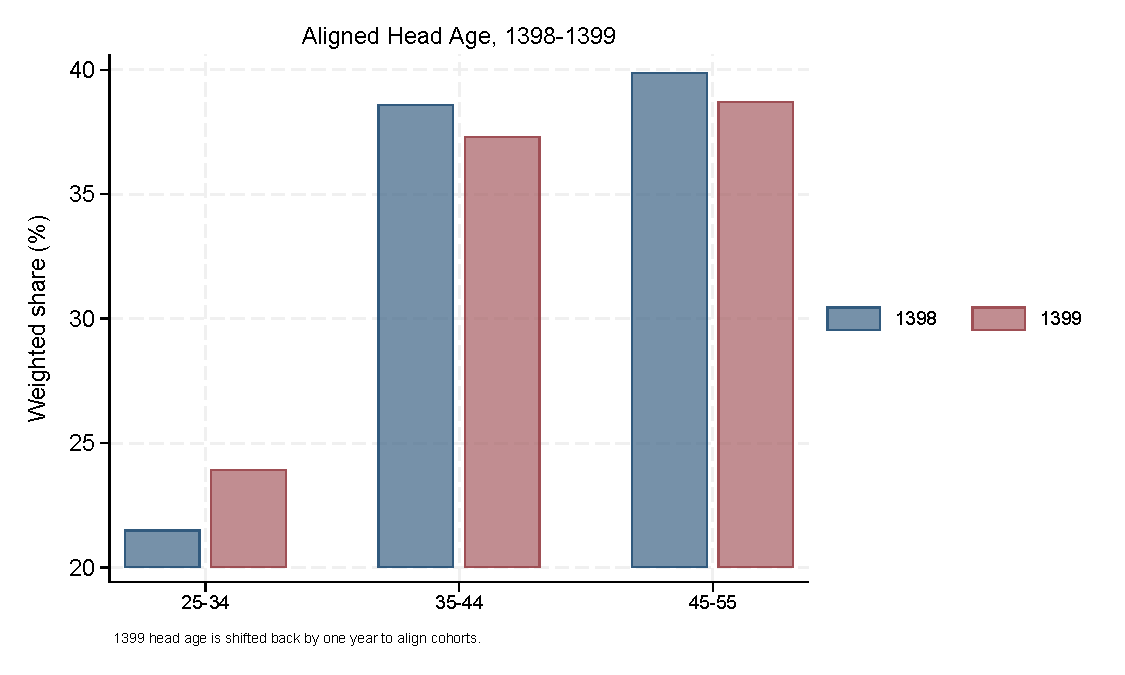
\includegraphics[width=0.85\linewidth]
    {Figures/population_stability_9899_age_barplot.pdf}
    \caption*{\scriptsize \textbf{Note:} The sample follows the all-household 1398-1399 specification. The 1399 head age is shifted back by one year to align the synthetic cohort with 1398.}
    \label{fig:population-stability-age}
\end{figure}

\begin{figure}[H]
    \centering
    \caption{Weighted Distribution of Household-Head Education, 1398-1399}
    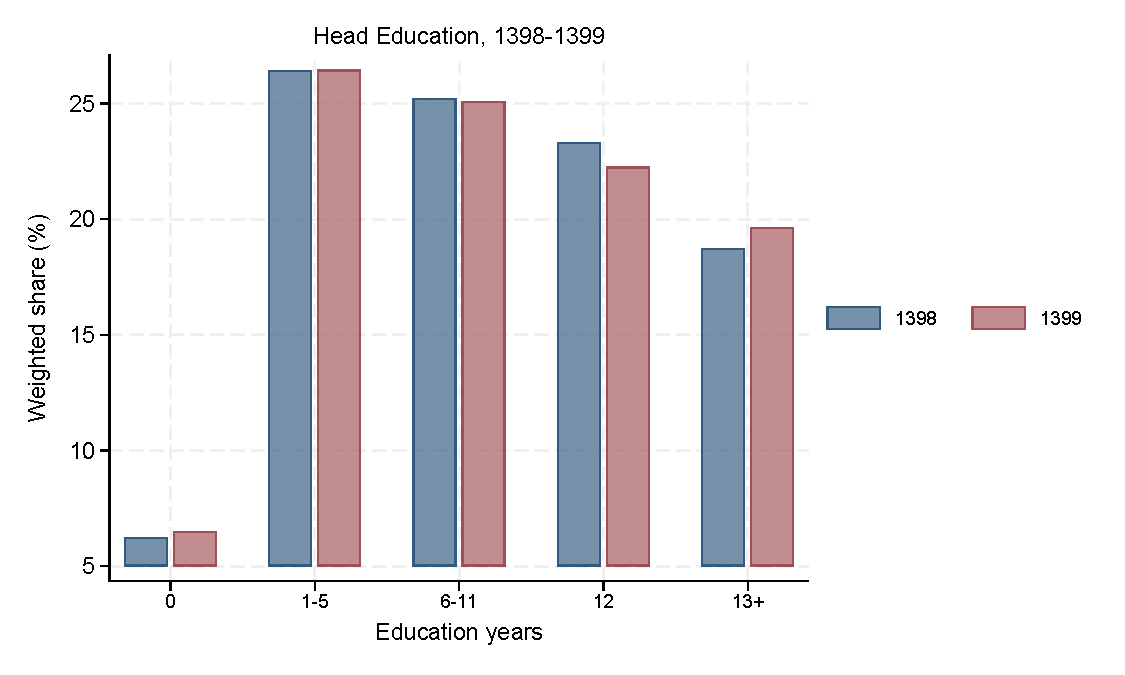
\includegraphics[width=0.85\linewidth]{Figures/population_stability_9899_education_barplot.pdf}
    \caption*{\scriptsize \textbf{Note:} Bars report weighted shares for the all-household age-aligned sample.}
    \label{fig:population-stability-education}
\end{figure}

\subsection{Residual Normality in the Consumption Models}
The parametric version of the synthetic-panel estimator relies on a distributional approximation for the regression errors. Following \citet{dang2014using}, we visually assess this assumption by comparing residuals from the all-household 1398 and 1399 consumption regressions with fitted normal densities. Figures \ref{fig:residual-normality-1398} and \ref{fig:residual-normality-1399} show the two diagnostic plots separately so that the residual distributions can be inspected more clearly.

\begin{figure}[H]
    \centering
    \caption{OLS Residuals and Fitted Normal Density, 1398}
    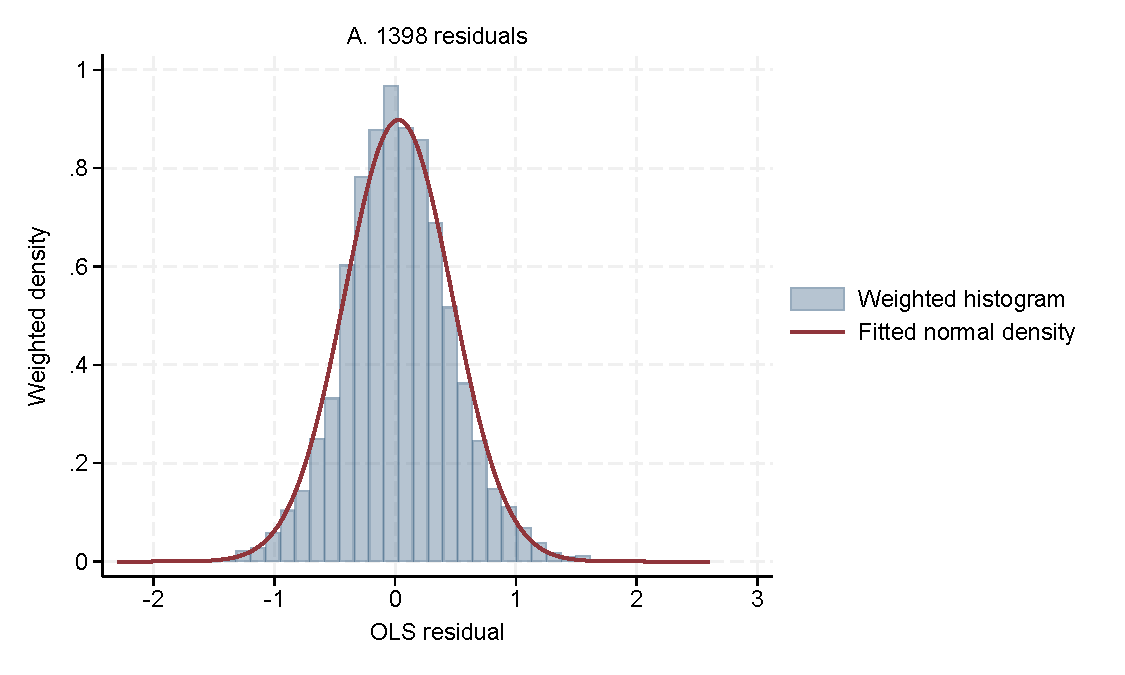
\includegraphics[width=0.85\linewidth]{Figures/residuals_1398_normality.pdf}
    \caption*{\scriptsize \textbf{Note:} Residuals are from the unweighted all-household OLS consumption model used for the 1398-1399 synthetic-panel estimates. The displayed density is weighted by HIES survey weights.}
    \label{fig:residual-normality-1398}
\end{figure}

\begin{figure}[H]
    \centering
    \caption{OLS Residuals and Fitted Normal Density, 1399}
    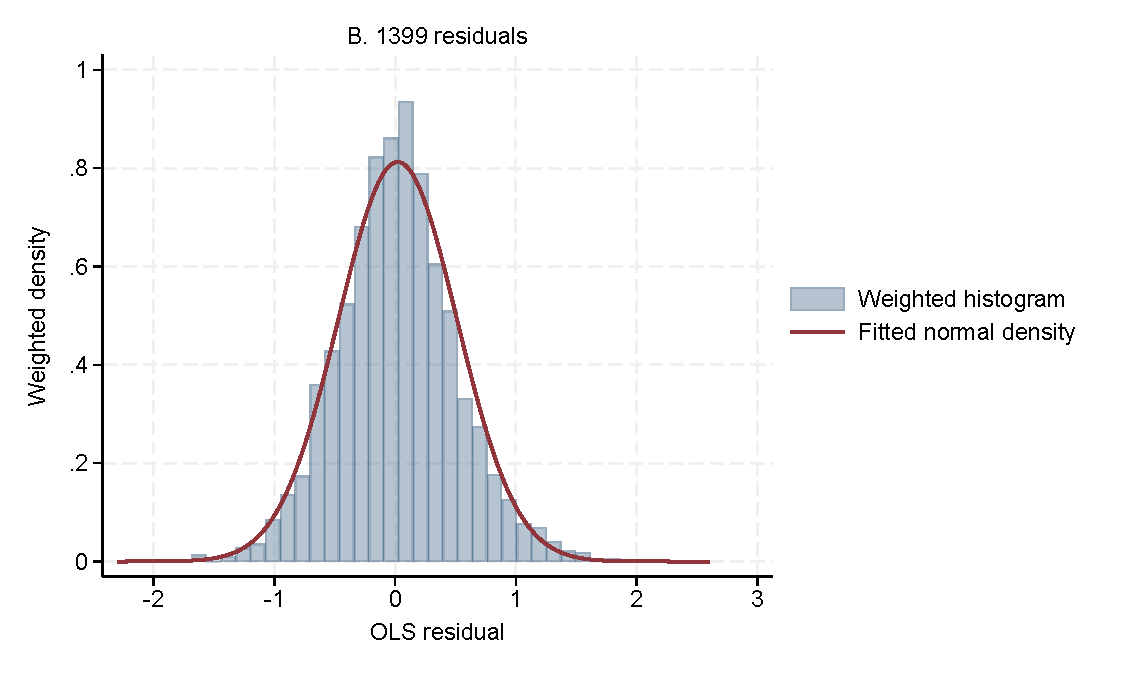
\includegraphics[width=0.85\linewidth]{Figures/residuals_1399_normality.pdf}
    \caption*{\scriptsize \textbf{Note:} Residuals are from the unweighted all-household OLS consumption model used for the 1398-1399 synthetic-panel estimates. The displayed density is weighted by HIES survey weights.}
    \label{fig:residual-normality-1399}
\end{figure}
\section{Potential Mechanisms}
The observed patterns in poverty dynamics - particularly the higher rates of chronic poverty among female-headed, less-educated, and rural households - can be understood through several interrelated economic and sociological mechanisms, grounded in the literature on poverty traps and vulnerability.
\textcolor{red}{we need  a histogram for non-labor earnings of households based on the households with higher and less than diploma educated heads and the household head's gender for two distinct years. }
First, the asset-based poverty trap framework, articulated by \citet{barrett2008poverty}, provides a foundational explanation. Households with limited initial endowments of physical, financial, or human capital may fall below a critical threshold, preventing investment in income - generating activities and locking them into persistent poverty. This mechanism is evident in our findings: households headed by individuals without university education lack the human capital necessary to access stable, formal - sector employment, consistent with the human capital theory of poverty \citep{schultz1961investment}. This lack of education constrains occupational mobility and resilience to economic shocks, as noted in studies from developing contexts \citep{behrman1999labor}.

Second, structural and labor market inequalities drive the gendered and spatial dimensions of our results. Female - headed households face a compounded disadvantage due to occupational segregation, wage discrimination, and the disproportionate burden of unpaid care work \citep{worldbank2012world}. Their overrepresentation in the informal sector, characterized by low pay and job insecurity \citep{ilostat2020women}, limits their capacity to accumulate savings or assets, increasing vulnerability to chronic poverty. This aligns with feminist political economy critiques that highlight how labor markets reproduce gendered poverty \citep{elson1999male}.

Third, the stark rural - urban divide can be attributed to spatial poverty traps. Rural households often depend on climate-sensitive agriculture, face higher transportation costs, and have limited access to financial services, quality education, and non-farm employment \citep{jalan2002geographic}. This geographic disadvantage is exacerbated by infrastructure deficits and public service concentration in urban areas, a common feature in middle-income countries \citep{kanbur2014urbanization}. The lower mobility out of poverty in rural areas reflects this structural constraint on economic diversification and opportunity.

Fourth, the broader macroeconomic and institutional context of Iran during the study period (2019-2020) serves as a critical precipitating mechanism. The confluence of stringent economic sanctions and the COVID-19 pandemic induced severe inflationary pressures, currency depreciation, and contraction in formal employment \citep{amid2021sanctions}. Such macroeconomic shocks disproportionately affect the most vulnerable groups—those with precarious employment, limited savings, and less diversified income sources—pushing transient poor households into chronic poverty and making escape more difficult for those already poor \citep{dercon2005vulnerability}. The shock likely eroded the modest gains of those near the poverty line, a phenomenon documented in other crisis settings \citep{hallegatte2016shock}.

Finally, the limited mobility observed, especially among the vulnerable subgroups, may reflect weak social protection systems. Effective safety nets and active labor market policies can mitigate shocks and facilitate poverty exits \citep{barrientos2011social}. The insufficiency or limited coverage of such programs in Iran during this period may have left households exposed to income volatility without adequate buffers, reinforcing chronic poverty \citep{moradi2021welfare}.

In summary, the mechanisms driving our results are multifaceted, operating at the intersection of individual human capital deficits, structural market inequalities, geographic disparities, and adverse macroeconomic shocks. These factors interact to create and sustain the poverty traps evident in the data, particularly for the most marginalized segments of Iranian society.

\section{Conclusion}
In this research, we have presented a method for estimating poverty dynamics in the absence of suitable panel data. Specifically, we have employed the synthetic panel model proposed by \cite{dang2014using}. to estimate the first-round consumption of households surveyed in the second round. We have applied this method to data from the Expenditures and Income Survey (HIES) for the years 2019 and 2020 in Iran, which is a period of particular significance due to the COVID-19 pandemic and US sanctions. Our results indicate that a significant proportion of households, particularly female-headed households, households with non-university educated heads, and rural households, are trapped in chronic poverty. Furthermore, we have also found that the estimates of poverty dynamics obtained from our synthetic panel model are in close agreement with those obtained from true panel data, demonstrating the validity and usefulness of this approach. Overall, this research highlights the importance of measuring poverty dynamics, which can provide valuable information for the design and implementation of poverty reduction policies.


\section*{Declaration}
During the preparation of this work, the authors used DeepSeek in order to improve grammatical precision. After using this service, the authors reviewed and edited the content as needed and take full responsibility for the content of the publication.

\newpage
\bibliographystyle{chicago-fa}
\bibliography{myref.bib}

\appendix
\section{2020-2021}
\begin{table}[H]
    \scriptsize
    \centering
    \caption{Poverty dynamics for all rural and urban households}
    \label{tab:all_99_1400}
    \begin{tabular}{lccccccccc}
\toprule
Poverty Status
& \multicolumn{1}{c}{\shortstack{Nonparametric\\bound}}
& \multicolumn{3}{c}{Parametric lower bound}
& \multicolumn{1}{c}{Truth}
& \multicolumn{3}{c}{Parametric upper bound}
& \multicolumn{1}{c}{\shortstack{Nonparametric\\bound}} \\
\cmidrule(lr){3-5} \cmidrule(lr){7-9}
& & Spec. 1 & Spec. 2 & Spec. 3 & & Spec. 3 & Spec. 2 & Spec. 1 & \\
\midrule

Poor, poor
& 17.9 & 18.7 & 15.2 & 14.0 & 11.0 & 10.7 & 10.0 & 8.7 & 8.6 \\
Std. Dev.
&      &      &      &      & 0.4 &      &      &      &      \\
\addlinespace

Poor, nonpoor
& 0.9 & 1.0 & 4.5 & 5.7 & 8.7 & 9.0 & 9.7 & 11.0 & 10.8 \\
Std. Dev.
&     &     &     &     & 0.5 &     &     &     &     \\
\addlinespace

Nonpoor, poor
& 3.2 & 3.5 & 7.0 & 8.1 & 11.1 & 11.5 & 12.2 & 13.4 & 12.6 \\
Std. Dev.
&     &     &     &     & 0.6 &     &     &     &     \\
\addlinespace

Nonpoor, nonpoor
& 78.0 & 76.8 & 73.3 & 72.2 & 69.2 & 68.8 & 68.1 & 66.9 & 68.1 \\
Std. Dev.
&      &      &      &      & 0.7 &      &      &      &      \\
\midrule

N
& 5593 & 5593 & 5593 & 5593 & 11142 & 5593 & 5593 & 5593 & 5593 \\
\bottomrule
\end{tabular}

    \caption*{\scriptsize \textbf{Note:} 2020-2021 (1399-1400), Source: HIES. Subpopulation: whole sample}
\end{table}

\begin{table}[H]
    \scriptsize
    \centering
    \caption{Poverty dynamics for female-headed households.}
    \label{fh_99_1400}
    \begin{tabular}{lccccccccc}
\toprule
Poverty Status
& \multicolumn{1}{c}{\shortstack{Nonparametric\\bound}}
& \multicolumn{3}{c}{Parametric lower bound}
& \multicolumn{1}{c}{Truth}
& \multicolumn{3}{c}{Parametric upper bound}
& \multicolumn{1}{c}{\shortstack{Nonparametric\\bound}} \\
\cmidrule(lr){3-5} \cmidrule(lr){7-9}
& & Spec. 1 & Spec. 2 & Spec. 3 & & Spec. 3 & Spec. 2 & Spec. 1 & \\
\midrule

Poor, poor
& 16.9 & 21.2 & 18.7 & 17.8 & 15.5 & 14.7 & 14.1 & 12.9 & 11.9 \\
Std. Dev.
&      &      &      &      & 1.4 &      &      &      &      \\
\addlinespace

Poor, nonpoor
& 4.8 & 3.9 & 6.3 & 7.3 & 9.7 & 10.4 & 11.0 & 12.2 & 12.7 \\
Std. Dev.
&     &     &     &     & 1.8 &     &     &     &     \\
\addlinespace

Nonpoor, poor
& 5.2 & 4.8 & 7.3 & 8.2 & 10.5 & 11.3 & 11.9 & 13.1 & 10.2 \\
Std. Dev.
&     &     &     &     & 1.6 &     &     &     &     \\
\addlinespace

Nonpoor, nonpoor
& 73.1 & 70.1 & 67.7 & 66.7 & 64.3 & 63.6 & 63.0 & 61.8 & 65.2 \\
Std. Dev.
&      &      &      &      & 2.4 &      &      &      &      \\
\midrule

N
& 459 & 459 & 459 & 459 & 874 & 459 & 459 & 459 & 459 \\
\bottomrule
\end{tabular}

    \caption*{\scriptsize \textbf{Note:} 2020-2021 (1399-1400), Source: HIES. Subpopulation: Female headed households}
\end{table}

\begin{table}[H]
    \scriptsize
    \centering
    \caption{Poverty dynamics for households whose head lacks university education.}
    \label{no_educ_99_1400}
    \begin{tabular}{lccccccccc}
\toprule
Poverty Status
& \multicolumn{1}{c}{\shortstack{Nonparametric\\bound}}
& \multicolumn{3}{c}{Parametric lower bound}
& \multicolumn{1}{c}{Truth}
& \multicolumn{3}{c}{Parametric upper bound}
& \multicolumn{1}{c}{\shortstack{Nonparametric\\bound}} \\
\cmidrule(lr){3-5} \cmidrule(lr){7-9}
& & Spec. 1 & Spec. 2 & Spec. 3 & & Spec. 3 & Spec. 2 & Spec. 1 & \\
\midrule

Poor, poor
& 19.9 & 21.5 & 17.5 & 16.2 & 12.7 & 12.4 & 11.6 & 10.1 & 9.9 \\
Std. Dev.
&      &      &      &      & 0.5 &      &      &      &      \\
\addlinespace

Poor, nonpoor
& 1.2 & 1.1 & 5.1 & 6.4 & 9.9 & 10.3 & 11.0 & 12.5 & 12.5 \\
Std. Dev.
&     &     &     &     & 0.6 &     &     &     &     \\
\addlinespace

Nonpoor, poor
& 3.7 & 3.8 & 7.8 & 9.1 & 12.6 & 12.9 & 13.7 & 15.1 & 13.7 \\
Std. Dev.
&     &     &     &     & 0.6 &     &     &     &     \\
\addlinespace

Nonpoor, nonpoor
& 75.3 & 73.6 & 69.6 & 68.3 & 64.8 & 64.5 & 63.7 & 62.2 & 63.9 \\
Std. Dev.
&      &      &      &      & 0.9 &      &      &      &      \\
\midrule

N
& 4969 & 4969 & 4969 & 4969 & 9785 & 4969 & 4969 & 4969 & 4969 \\
\bottomrule
\end{tabular}

     \caption*{\scriptsize \textbf{Note:} 2020-2021 (1399-1400), Source: HIES. Subpopulation:  households' head with non-college education}
\end{table}

\begin{table}[H]
    \scriptsize
    \centering
    \caption{ Poverty dynamics for households with a university-educated head}
    \label{with_educ_99_1400}
    \begin{tabular}{lccccccccc}
\toprule
Poverty Status
& \multicolumn{1}{c}{\shortstack{Nonparametric\\bound}}
& \multicolumn{3}{c}{Parametric lower bound}
& \multicolumn{1}{c}{Truth}
& \multicolumn{3}{c}{Parametric upper bound}
& \multicolumn{1}{c}{\shortstack{Nonparametric\\bound}} \\
\cmidrule(lr){3-5} \cmidrule(lr){7-9}
& & Spec. 1 & Spec. 2 & Spec. 3 & & Spec. 3 & Spec. 2 & Spec. 1 & \\
\midrule

Poor, poor
& 2.0 & 2.8 & 2.1 & 1.8 & 1.1 & 1.0 & 0.9 & 0.6 & 0.5 \\
Std. Dev.
&      &      &      &      & 0.4 &      &      &      &      \\
\addlinespace

Poor, nonpoor
& 0.3 & 0.3 & 1.0 & 1.3 & 1.9 & 2.0 & 2.2 & 2.4 & 2.3 \\
Std. Dev.
&     &     &     &     & 0.6 &     &     &     &     \\
\addlinespace

Nonpoor, poor
& 2.5 & 2.8 & 3.6 & 3.8 & 4.5 & 4.6 & 4.8 & 5.0 & 4.0 \\
Std. Dev.
&     &     &     &     & 1.0 &     &     &     &     \\
\addlinespace

Nonpoor, nonpoor
& 95.2 & 94.1 & 93.4 & 93.1 & 92.4 & 92.3 & 92.2 & 91.9 & 93.2 \\
Std. Dev.
&      &      &      &      & 1.2 &      &      &      &      \\
\midrule

N
& 664 & 664 & 664 & 664 & 1346 & 664 & 664 & 664 & 664 \\
\bottomrule
\end{tabular}

        \caption*{\scriptsize \textbf{Note:} 2020-2021 (1399-1400), Source: HIES. Subpopulation:  households' head with college education}
\end{table}

\begin{table}[H]
    \scriptsize
    \centering
    \caption{Poverty dynamics of urban households.}
    \label{urban_1399_1400}
   \begin{tabular}{lccccccccc}
\toprule
Poverty Status
& \multicolumn{1}{c}{\shortstack{Nonparametric\\bound}}
& \multicolumn{3}{c}{Parametric lower bound}
& \multicolumn{1}{c}{Truth}
& \multicolumn{3}{c}{Parametric upper bound}
& \multicolumn{1}{c}{\shortstack{Nonparametric\\bound}} \\
\cmidrule(lr){3-5} \cmidrule(lr){7-9}
& & Spec. 1 & Spec. 2 & Spec. 3 & & Spec. 3 & Spec. 2 & Spec. 1 & \\
\midrule

Poor, poor
& 10.4 & 12.1 & 9.5 & 8.6 & 6.3 & 6.0 & 5.5 & 4.5 & 4.0 \\
Std. Dev.
&      &      &      &      & 0.5 &      &      &      &      \\
\addlinespace

Poor, nonpoor
& 1.4 & 1.3 & 3.9 & 4.8 & 7.1 & 7.4 & 7.9 & 8.8 & 9.1 \\
Std. Dev.
&     &     &     &     & 0.6 &     &     &     &     \\
\addlinespace

Nonpoor, poor
& 2.5 & 3.0 & 5.6 & 6.5 & 8.8 & 9.1 & 9.6 & 10.5 & 8.9 \\
Std. Dev.
&     &     &     &     & 0.6 &     &     &     &     \\
\addlinespace

Nonpoor, nonpoor
& 85.7 & 83.7 & 81.0 & 80.1 & 77.8 & 77.5 & 77.0 & 76.1 & 78.0 \\
Std. Dev.
&      &      &      &      & 0.8 &      &      &      &      \\
\midrule

N
& 2865 & 2865 & 2865 & 2865 & 5616 & 2865 & 2865 & 2865 & 2865 \\
\bottomrule
\end{tabular}

            \caption*{\scriptsize \textbf{Note:}  This table illustrates that between 2020 and 2021.  1. Poverty rates in percent are calculated using HIES data, statistical Center of Iran, and predictions obtained using data in the second survey rounds.
Full regression results are provided in Tables 2.1a and 2.1b in Appendix ??. \\
2. All calculations are weighted using population weights for each survey round. Standard errors in parentheses.\\
3. Number of replications for the estimates is 500.\\
4. Specification 1 uses $\rho_H=1$ and $\rho_S=0$ for the lower and upper bounds, respectively, and is the parametric analogue of the nonparametric bounds. Specification 2
uses $\rho_H=0.8$ and $\rho_S=0.2$, and Specification 3 uses $\rho_H=0.7$ and $\rho_S=0.3$ for the lower and upper bounds, respectively. The regressors in all regressions are the
same as in Model 1 in Table 1 plus an urban/rural dummy variable.
5. Household heads' ages are restricted to between 25 and 55 in the first survey round.}
\end{table}

\begin{table}[H]
    \scriptsize
    \centering
    \caption{Poverty dynamics of rural households}
    \label{rural_1399_1400}
   \begin{tabular}{lccccccccc}
\toprule
Poverty Status
& \multicolumn{1}{c}{\shortstack{Nonparametric\\bound}}
& \multicolumn{3}{c}{Parametric lower bound}
& \multicolumn{1}{c}{Truth}
& \multicolumn{3}{c}{Parametric upper bound}
& \multicolumn{1}{c}{\shortstack{Nonparametric\\bound}} \\
\cmidrule(lr){3-5} \cmidrule(lr){7-9}
& & Spec. 1 & Spec. 2 & Spec. 3 & & Spec. 3 & Spec. 2 & Spec. 1 & \\
\midrule

Poor, poor
& 36.5 & 36.3 & 31.3 & 29.6 & 24.4 & 24.4 & 23.3 & 21.2 & 21.9 \\
Std. Dev.
&      &      &      &      & 0.8 &      &      &      &      \\
\addlinespace

Poor, nonpoor
& 2.6 & 2.5 & 7.5 & 9.2 & 14.2 & 14.4 & 15.5 & 17.6 & 17.2 \\
Std. Dev.
&     &     &     &     & 0.8 &     &     &     &     \\
\addlinespace

Nonpoor, poor
& 4.5 & 4.4 & 9.4 & 11.1 & 16.2 & 16.3 & 17.4 & 19.5 & 19.1 \\
Std. Dev.
&     &     &     &     & 0.8 &     &     &     &     \\
\addlinespace

Nonpoor, nonpoor
& 56.4 & 56.8 & 51.8 & 50.1 & 45.1 & 44.9 & 43.8 & 41.7 & 41.8 \\
Std. Dev.
&      &      &      &      & 1.0 &      &      &      &      \\
\midrule

N
& 2832 & 2832 & 2832 & 2832 & 5526 & 2832 & 2832 & 2832 & 2832 \\
\bottomrule
\end{tabular}

            \caption*{\scriptsize \textbf{Note:} 2020-2021 (1399-1400), Source: HIES. Subpopulation:  Rural area}
\end{table}

\section{2021-2022}
\begin{table}[H]
    \scriptsize
    \centering
    \caption{ Poverty dynamics for all rural and urban households}
    \label{all_1400-1401}
   \begin{tabular}{lccccccccc}
\toprule
Poverty Status
& \multicolumn{1}{c}{\shortstack{Nonparametric\\bound}}
& \multicolumn{3}{c}{Parametric lower bound}
& \multicolumn{1}{c}{Truth}
& \multicolumn{3}{c}{Parametric upper bound}
& \multicolumn{1}{c}{\shortstack{Nonparametric\\bound}} \\
\cmidrule(lr){3-5} \cmidrule(lr){7-9}
& & Spec. 1 & Spec. 2 & Spec. 3 & & Spec. 3 & Spec. 2 & Spec. 1 & \\
\midrule

Poor, poor
& 17.0 & 18.0 & 14.4 & 13.3 & 9.7 & 9.9 & 9.2 & 8.0 & 7.8 \\
Std. Dev.
&      &      &      &      & 0.4 &      &      &      &      \\
\addlinespace

Poor, nonpoor
& 3.3 & 3.3 & 7.0 & 8.1 & 11.6 & 11.4 & 12.1 & 13.3 & 13.1 \\
Std. Dev.
&     &     &     &     & 0.6 &     &     &     &     \\
\addlinespace

Nonpoor, poor
& 0.6 & 0.9 & 4.5 & 5.7 & 9.2 & 9.0 & 9.7 & 10.9 & 9.7 \\
Std. Dev.
&     &     &     &     & 0.5 &     &     &     &     \\
\addlinespace

Nonpoor, nonpoor
& 79.1 & 77.7 & 74.1 & 73.0 & 69.5 & 69.6 & 69.0 & 67.7 & 69.3 \\
Std. Dev.
&      &      &      &      & 0.7 &      &      &      &      \\
\midrule

N
& 5582 & 5582 & 5582 & 5582 & 11008 & 5582 & 5582 & 5582 & 5582 \\
\bottomrule
\end{tabular}

    \caption*{\scriptsize \textbf{Note:} 2021-2022 (1400-1401), Source: HIES. Subpopulation:  Whole sample}
\end{table}

\begin{table}[H]
    \scriptsize
    \centering
    \caption{Poverty dynamics for female-headed households.}
    \label{fh_1400_1401}
    \begin{tabular}{lccccccccc}
\toprule
Poverty Status
& \multicolumn{1}{c}{\shortstack{Nonparametric\\bound}}
& \multicolumn{3}{c}{Parametric lower bound}
& \multicolumn{1}{c}{Truth}
& \multicolumn{3}{c}{Parametric upper bound}
& \multicolumn{1}{c}{\shortstack{Nonparametric\\bound}} \\
\cmidrule(lr){3-5} \cmidrule(lr){7-9}
& & Spec. 1 & Spec. 2 & Spec. 3 & & Spec. 3 & Spec. 2 & Spec. 1 & \\
\midrule

Poor, poor
& 21.6 & 21.9 & 19.3 & 18.2 & 15.2 & 15.0 & 14.3 & 13.1 & 12.5 \\
Std. Dev.
&      &      &      &      & 1.6 &      &      &      &      \\
\addlinespace

Poor, nonpoor
& 7.3 & 7.1 & 9.7 & 10.8 & 13.7 & 14.0 & 14.7 & 15.9 & 16.0 \\
Std. Dev.
&     &     &     &     & 2.0 &     &     &     &     \\
\addlinespace

Nonpoor, poor
& 1.4 & 1.7 & 4.4 & 5.4 & 8.4 & 8.6 & 9.3 & 10.6 & 10.4 \\
Std. Dev.
&     &     &     &     & 1.7 &     &     &     &     \\
\addlinespace

Nonpoor, nonpoor
& 69.7 & 69.3 & 66.6 & 65.6 & 62.6 & 62.4 & 61.7 & 60.4 & 61.0 \\
Std. Dev.
&      &      &      &      & 2.5 &      &      &      &      \\
\midrule

N
& 439 & 439 & 439 & 439 & 849 & 439 & 439 & 439 & 439 \\
\bottomrule
\end{tabular}

      \caption*{\scriptsize \textbf{Note:} 1400-1401, 2021-2022.  This table illustrates that between 2021 and 2022.  1. Poverty rates in percent are calculated using HIES data, statistical Center of Iran, and predictions obtained using data in the second survey rounds.
Full regression results are provided in Tables 2.1a and 2.1b in Appendix ??. \\
2. All calculations are weighted using population weights for each survey round. Standard errors in parentheses.\\
3. Number of replications for the estimates is 500.\\
4. Specification 1 uses $\rho_H=1$ and $\rho_S=0$ for the lower and upper bounds, respectively, and is the parametric analogue of the nonparametric bounds. Specification 2
uses $\rho_H=0.8$ and $\rho_S=0.2$, and Specification 3 uses $\rho_H=0.7$ and $\rho_S=0.3$ for the lower and upper bounds, respectively. The regressors in all regressions are the
same as in Model 1 in Table 1 plus an urban/rural dummy variable.
5. Household heads' ages are restricted to between 25 and 55 in the first survey round.}
\end{table}


\begin{table}[H]
    \scriptsize
    \centering
    \caption{Poverty dynamics for households whose head lacks university education}
    \label{no_educ_1400_1401}
   \begin{tabular}{lccccccccc}
\toprule
Poverty Status
& \multicolumn{1}{c}{\shortstack{Nonparametric\\bound}}
& \multicolumn{3}{c}{Parametric lower bound}
& \multicolumn{1}{c}{Truth}
& \multicolumn{3}{c}{Parametric upper bound}
& \multicolumn{1}{c}{\shortstack{Nonparametric\\bound}} \\
\cmidrule(lr){3-5} \cmidrule(lr){7-9}
& & Spec. 1 & Spec. 2 & Spec. 3 & & Spec. 3 & Spec. 2 & Spec. 1 & \\
\midrule

Poor, poor
& 18.0 & 19.8 & 16.1 & 14.9 & 10.8 & 11.2 & 10.4 & 9.0 & 8.6 \\
Std. Dev.
&      &      &      &      & 0.5 &      &      &      &      \\
\addlinespace

Poor, nonpoor
& 5.0 & 4.9 & 8.7 & 9.9 & 13.9 & 13.6 & 14.4 & 15.7 & 15.8 \\
Std. Dev.
&     &     &     &     & 0.7 &     &     &     &     \\
\addlinespace

Nonpoor, poor
& 0.5 & 0.5 & 4.2 & 5.5 & 9.4 & 9.2 & 9.9 & 11.3 & 10.0 \\
Std. Dev.
&     &     &     &     & 0.6 &     &     &     &     \\
\addlinespace

Nonpoor, nonpoor
& 76.4 & 74.7 & 71.0 & 69.8 & 65.8 & 66.1 & 65.3 & 63.9 & 65.7 \\
Std. Dev.
&      &      &      &      & 0.8 &      &      &      &      \\
\midrule

N
& 4871 & 4871 & 4871 & 4871 & 9650 & 4871 & 4871 & 4871 & 4871 \\
\bottomrule
\end{tabular}

          \caption*{\scriptsize \textbf{Note:} 1400-1401.}
\end{table}


\begin{table}[H]
    \scriptsize
    \centering
    \caption{ Poverty dynamics for households with a university-educated head}
    \label{have_educ_1400_1401}
   \begin{tabular}{lccccccccc}
\toprule
Poverty Status
& \multicolumn{1}{c}{\shortstack{Nonparametric\\bound}}
& \multicolumn{3}{c}{Parametric lower bound}
& \multicolumn{1}{c}{Truth}
& \multicolumn{3}{c}{Parametric upper bound}
& \multicolumn{1}{c}{\shortstack{Nonparametric\\bound}} \\
\cmidrule(lr){3-5} \cmidrule(lr){7-9}
& & Spec. 1 & Spec. 2 & Spec. 3 & & Spec. 3 & Spec. 2 & Spec. 1 & \\
\midrule

Poor, poor
& 2.9 & 3.9 & 2.8 & 2.4 & 1.5 & 1.4 & 1.2 & 0.9 & 0.9 \\
Std. Dev.
&      &      &      &      & 0.5 &      &      &      &      \\
\addlinespace

Poor, nonpoor
& 0.6 & 1.0 & 2.1 & 2.4 & 3.4 & 3.4 & 3.6 & 4.0 & 3.5 \\
Std. Dev.
&     &     &     &     & 0.8 &     &     &     &     \\
\addlinespace

Nonpoor, poor
& 0.7 & 2.0 & 3.1 & 3.5 & 4.4 & 4.5 & 4.7 & 5.0 & 2.8 \\
Std. Dev.
&     &     &     &     & 0.9 &     &     &     &     \\
\addlinespace

Nonpoor, nonpoor
& 95.7 & 93.1 & 92.0 & 91.7 & 90.7 & 90.6 & 90.5 & 90.1 & 92.8 \\
Std. Dev.
&      &      &      &      & 1.2 &      &      &      &      \\
\midrule

N
& 720 & 720 & 720 & 720 & 1362 & 720 & 720 & 720 & 720 \\
\bottomrule
\end{tabular}

      \caption*{\scriptsize \textbf{Note:} 1400-1401.  This table illustrates that between 2021 and 2022.  1. Poverty rates in percent are calculated using HIES data, statistical Center of Iran, and predictions obtained using data in the second survey rounds.
Full regression results are provided in Tables 2.1a and 2.1b in Appendix ??. \\
2. All calculations are weighted using population weights for each survey round. Standard errors in parentheses.\\
3. Number of replications for the estimates is 500.\\
4. Specification 1 uses $\rho_H=1$ and $\rho_S=0$ for the lower and upper bounds, respectively, and is the parametric analogue of the nonparametric bounds. Specification 2
uses $\rho_H=0.8$ and $\rho_S=0.2$, and Specification 3 uses $\rho_H=0.7$ and $\rho_S=0.3$ for the lower and upper bounds, respectively. The regressors in all regressions are the
same as in Model 1 in Table 1 plus an urban/rural dummy variable.
5. Household heads' ages are restricted to between 25 and 55 in the first survey round.}
\end{table}


\begin{table}[H]
    \scriptsize
    \centering
    \caption{Poverty dynamics of urban households.}
    \label{urban_1400_1401}
    \begin{tabular}{lccccccccc}
\toprule
Poverty Status
& \multicolumn{1}{c}{\shortstack{Nonparametric\\bound}}
& \multicolumn{3}{c}{Parametric lower bound}
& \multicolumn{1}{c}{Truth}
& \multicolumn{3}{c}{Parametric upper bound}
& \multicolumn{1}{c}{\shortstack{Nonparametric\\bound}} \\
\cmidrule(lr){3-5} \cmidrule(lr){7-9}
& & Spec. 1 & Spec. 2 & Spec. 3 & & Spec. 3 & Spec. 2 & Spec. 1 & \\
\midrule

Poor, poor
& 9.5 & 11.7 & 8.9 & 8.0 & 5.3 & 5.4 & 4.8 & 3.9 & 3.3 \\
Std. Dev.
&      &      &      &      & 0.5 &      &      &      &      \\
\addlinespace

Poor, nonpoor
& 3.1 & 2.7 & 5.6 & 6.5 & 9.2 & 9.1 & 9.6 & 10.6 & 10.7 \\
Std. Dev.
&     &     &     &     & 0.7 &     &     &     &     \\
\addlinespace

Nonpoor, poor
& 0.9 & 1.3 & 4.1 & 5.0 & 7.6 & 7.6 & 8.2 & 9.1 & 7.1 \\
Std. Dev.
&     &     &     &     & 0.7 &     &     &     &     \\
\addlinespace

Nonpoor, nonpoor
& 86.5 & 84.3 & 81.4 & 80.5 & 78.0 & 77.9 & 77.4 & 76.5 & 78.9 \\
Std. Dev.
&      &      &      &      & 0.9 &      &      &      &      \\
\midrule

N
& 2845 & 2845 & 2845 & 2845 & 5601 & 2845 & 2845 & 2845 & 2845 \\
\bottomrule
\end{tabular}

        \caption*{\scriptsize \textbf{Note:} 1400-1401. 2021-2022, Source: HIES. Subpopulation:  Urban area}
\end{table}

\begin{table}[H]
    \scriptsize
    \centering
    \caption{Poverty dynamics of rural households.}
    \label{rural_1400_1401}
    \begin{tabular}{lccccccccc}
\toprule
Poverty Status
& \multicolumn{1}{c}{\shortstack{Nonparametric\\bound}}
& \multicolumn{3}{c}{Parametric lower bound}
& \multicolumn{1}{c}{Truth}
& \multicolumn{3}{c}{Parametric upper bound}
& \multicolumn{1}{c}{\shortstack{Nonparametric\\bound}} \\
\cmidrule(lr){3-5} \cmidrule(lr){7-9}
& & Spec. 1 & Spec. 2 & Spec. 3 & & Spec. 3 & Spec. 2 & Spec. 1 & \\
\midrule

Poor, poor
& 35.9 & 34.6 & 29.6 & 27.9 & 21.9 & 22.7 & 21.6 & 19.6 & 20.7 \\
Std. Dev.
&      &      &      &      & 0.8 &      &      &      &      \\
\addlinespace

Poor, nonpoor
& 5.8 & 5.6 & 10.6 & 12.3 & 18.3 & 17.5 & 18.5 & 20.6 & 19.7 \\
Std. Dev.
&     &     &     &     & 0.9 &     &     &     &     \\
\addlinespace

Nonpoor, poor
& 1.7 & 1.5 & 6.5 & 8.2 & 14.0 & 13.3 & 14.4 & 16.5 & 17.0 \\
Std. Dev.
&     &     &     &     & 0.8 &     &     &     &     \\
\addlinespace

Nonpoor, nonpoor
& 56.6 & 58.3 & 53.3 & 51.6 & 45.8 & 46.5 & 45.4 & 43.3 & 42.6 \\
Std. Dev.
&      &      &      &      & 1.0 &      &      &      &      \\
\midrule

N
& 2754 & 2754 & 2754 & 2754 & 5402 & 2754 & 2754 & 2754 & 2754 \\
\bottomrule
\end{tabular}

       \caption*{\scriptsize \textbf{Note:}  1400-1401. 2021-2022, Source: HIES. Subpopulation:  Rural area}
\end{table}


\begin{table}[H]
    \scriptsize
    \centering
    \caption{ Poverty dynamics for all rural and urban households}
    \label{all_1401_1402}
   \begin{tabular}{lccccccccc}
\toprule
Poverty Status
& \multicolumn{1}{c}{\shortstack{Nonparametric\\bound}}
& \multicolumn{3}{c}{Parametric lower bound}
& \multicolumn{1}{c}{Truth}
& \multicolumn{3}{c}{Parametric upper bound}
& \multicolumn{1}{c}{\shortstack{Nonparametric\\bound}} \\
\cmidrule(lr){3-5} \cmidrule(lr){7-9}
& & Spec. 1 & Spec. 2 & Spec. 3 & & Spec. 3 & Spec. 2 & Spec. 1 & \\
\midrule

Poor, poor
& 11.1 & 12.9 & 10.7 & 9.9 & 7.4 & 7.3 & 6.8 & 5.8 & 5.4 \\
Std. Dev.
&      &      &      &      & 0.4 &      &      &      &      \\
\addlinespace

Poor, nonpoor
& 5.8 & 6.1 & 8.3 & 9.2 & 11.7 & 11.8 & 12.3 & 13.3 & 13.3 \\
Std. Dev.
&     &     &     &     & 0.6 &     &     &     &     \\
\addlinespace

Nonpoor, poor
& 0.6 & 0.7 & 2.8 & 3.7 & 6.2 & 6.3 & 6.8 & 7.8 & 6.3 \\
Std. Dev.
&     &     &     &     & 0.4 &     &     &     &     \\
\addlinespace

Nonpoor, nonpoor
& 82.5 & 80.3 & 78.1 & 77.3 & 74.7 & 74.6 & 74.1 & 73.1 & 75.0 \\
Std. Dev.
&      &      &      &      & 0.7 &      &      &      &      \\
\midrule

N
& 5448 & 5448 & 5448 & 5448 & 10755 & 5448 & 5448 & 5448 & 5448 \\
\bottomrule
\end{tabular}

      \caption*{\scriptsize \textbf{Note:} 1400-1401.  This table illustrates that between 2021 and 2022.  1. Poverty rates in percent are calculated using HIES data, statistical Center of Iran, and predictions obtained using data in the second survey rounds.
Full regression results are provided in Tables 2.1a and 2.1b in Appendix ??. \\
2. All calculations are weighted using population weights for each survey round. Standard errors in parentheses.\\
3. Number of replications for the estimates is 500.\\
4. Specification 1 uses $\rho_H=1$ and $\rho_S=0$ for the lower and upper bounds, respectively, and is the parametric analogue of the nonparametric bounds. Specification 2
uses $\rho_H=0.8$ and $\rho_S=0.2$, and Specification 3 uses $\rho_H=0.7$ and $\rho_S=0.3$ for the lower and upper bounds, respectively. The regressors in all regressions are the
same as in Model 1 in Table 1 plus an urban/rural dummy variable.
5. Household heads' ages are restricted to between 25 and 55 in the first survey round.}
\end{table}
\section{2022-2023}
\begin{table}[H]
    \scriptsize
    \centering
    \caption{Poverty dynamics for female-headed households}
    \label{fh_1401_1402}
    \begin{tabular}{lccccccccc}
\toprule
Poverty Status
& \multicolumn{1}{c}{\shortstack{Nonparametric\\bound}}
& \multicolumn{3}{c}{Parametric lower bound}
& \multicolumn{1}{c}{Truth}
& \multicolumn{3}{c}{Parametric upper bound}
& \multicolumn{1}{c}{\shortstack{Nonparametric\\bound}} \\
\cmidrule(lr){3-5} \cmidrule(lr){7-9}
& & Spec. 1 & Spec. 2 & Spec. 3 & & Spec. 3 & Spec. 2 & Spec. 1 & \\
\midrule

Poor, poor
& 14.8 & 15.2 & 13.1 & 12.3 & 10.4 & 9.7 & 9.2 & 8.2 & 8.2 \\
Std. Dev.
&      &      &      &      & 1.3 &      &      &      &      \\
\addlinespace

Poor, nonpoor
& 9.3 & 6.5 & 8.6 & 9.4 & 11.3 & 12.0 & 12.5 & 13.5 & 12.9 \\
Std. Dev.
&     &     &     &     & 1.7 &     &     &     &     \\
\addlinespace

Nonpoor, poor
& 2.1 & 1.9 & 4.0 & 4.8 & 6.8 & 7.4 & 7.9 & 8.9 & 8.7 \\
Std. Dev.
&     &     &     &     & 1.4 &     &     &     &     \\
\addlinespace

Nonpoor, nonpoor
& 73.9 & 76.4 & 74.3 & 73.5 & 71.5 & 70.9 & 70.4 & 69.4 & 70.2 \\
Std. Dev.
&      &      &      &      & 2.2 &      &      &      &      \\
\midrule

N
& 460 & 460 & 460 & 460 & 880 & 460 & 460 & 460 & 460 \\
\bottomrule
\end{tabular}

    \caption*{\scriptsize \textbf{Note:} 1401-1402.  This table illustrates that between 2022 and 2023.  1. Poverty rates in percent are calculated using HIES data, statistical Center of Iran, and predictions obtained using data in the second survey rounds.
Full regression results are provided in Tables 2.1a and 2.1b in Appendix ??. \\
2. All calculations are weighted using population weights for each survey round. Standard errors in parentheses.\\
3. Number of replications for the estimates is 500.\\
4. Specification 1 uses $\rho_H=1$ and $\rho_S=0$ for the lower and upper bounds, respectively, and is the parametric analogue of the nonparametric bounds. Specification 2
uses $\rho_H=0.8$ and $\rho_S=0.2$, and Specification 3 uses $\rho_H=0.7$ and $\rho_S=0.3$ for the lower and upper bounds, respectively. The regressors in all regressions are the
same as in Model 1 in Table 1 plus an urban/rural dummy variable.
5. Household heads' ages are restricted to between 25 and 55 in the first survey round.}
\end{table}

\begin{table}[H]
    \scriptsize
    \centering
    \caption{ Poverty dynamics for households whose head lacks university educa-
tion}
    \label{no_educ_1401_1402}
   \begin{tabular}{lccccccccc}
\toprule
Poverty Status
& \multicolumn{1}{c}{\shortstack{Nonparametric\\bound}}
& \multicolumn{3}{c}{Parametric lower bound}
& \multicolumn{1}{c}{Truth}
& \multicolumn{3}{c}{Parametric upper bound}
& \multicolumn{1}{c}{\shortstack{Nonparametric\\bound}} \\
\cmidrule(lr){3-5} \cmidrule(lr){7-9}
& & Spec. 1 & Spec. 2 & Spec. 3 & & Spec. 3 & Spec. 2 & Spec. 1 & \\
\midrule

Poor, poor
& 13.0 & 14.9 & 12.5 & 11.5 & 8.6 & 8.5 & 7.9 & 6.8 & 6.5 \\
Std. Dev.
&      &      &      &      & 0.4 &      &      &      &      \\
\addlinespace

Poor, nonpoor
& 6.5 & 6.8 & 9.3 & 10.3 & 13.2 & 13.3 & 13.9 & 15.0 & 14.8 \\
Std. Dev.
&     &     &     &     & 0.6 &     &     &     &     \\
\addlinespace

Nonpoor, poor
& 0.4 & 0.5 & 3.0 & 3.9 & 6.8 & 6.9 & 7.6 & 8.7 & 7.0 \\
Std. Dev.
&     &     &     &     & 0.5 &     &     &     &     \\
\addlinespace

Nonpoor, nonpoor
& 80.0 & 77.7 & 75.3 & 74.3 & 71.4 & 71.3 & 70.7 & 69.6 & 71.7 \\
Std. Dev.
&      &      &      &      & 0.8 &      &      &      &      \\
\midrule

N
& 4789 & 4789 & 4789 & 4789 & 9416 & 4789 & 4789 & 4789 & 4789 \\
\bottomrule
\end{tabular}

     \caption*{\scriptsize \textbf{Note:} 1401-1402.}
\end{table}

\begin{table}[H]
    \scriptsize
    \centering
    \caption{ Poverty dynamics for households with a university-educated head}
    \label{with_educ_1401_1402}
    \begin{tabular}{lccccccccc}
\toprule
Poverty Status
& \multicolumn{1}{c}{\shortstack{Nonparametric\\bound}}
& \multicolumn{3}{c}{Parametric lower bound}
& \multicolumn{1}{c}{Truth}
& \multicolumn{3}{c}{Parametric upper bound}
& \multicolumn{1}{c}{\shortstack{Nonparametric\\bound}} \\
\cmidrule(lr){3-5} \cmidrule(lr){7-9}
& & Spec. 1 & Spec. 2 & Spec. 3 & & Spec. 3 & Spec. 2 & Spec. 1 & \\
\midrule

Poor, poor
& 1.8 & 2.2 & 1.6 & 1.3 & 0.7 & 0.7 & 0.6 & 0.4 & 0.2 \\
Std. Dev.
&      &      &      &      & 0.4 &      &      &      &      \\
\addlinespace

Poor, nonpoor
& 1.1 & 1.9 & 2.6 & 2.8 & 3.4 & 3.4 & 3.5 & 3.7 & 3.6 \\
Std. Dev.
&     &     &     &     & 0.8 &     &     &     &     \\
\addlinespace

Nonpoor, poor
& 0.3 & 0.6 & 1.3 & 1.5 & 2.0 & 2.1 & 2.2 & 2.4 & 1.9 \\
Std. Dev.
&     &     &     &     & 0.7 &     &     &     &     \\
\addlinespace

Nonpoor, nonpoor
& 96.8 & 95.3 & 94.6 & 94.4 & 93.9 & 93.7 & 93.6 & 93.4 & 94.3 \\
Std. Dev.
&      &      &      &      & 1.1 &      &      &      &      \\
\midrule

N
& 689 & 689 & 689 & 689 & 1348 & 689 & 689 & 689 & 689 \\
\bottomrule
\end{tabular}

         \caption*{\scriptsize \textbf{Note:} 1401-1402.}
\end{table}

\begin{table}[H]
    \scriptsize
    \centering
    \caption{Poverty dynamics of urban households.}
    \label{urban_1401_1402}
   \begin{tabular}{lccccccccc}
\toprule
Poverty Status
& \multicolumn{1}{c}{\shortstack{Nonparametric\\bound}}
& \multicolumn{3}{c}{Parametric lower bound}
& \multicolumn{1}{c}{Truth}
& \multicolumn{3}{c}{Parametric upper bound}
& \multicolumn{1}{c}{\shortstack{Nonparametric\\bound}} \\
\cmidrule(lr){3-5} \cmidrule(lr){7-9}
& & Spec. 1 & Spec. 2 & Spec. 3 & & Spec. 3 & Spec. 2 & Spec. 1 & \\
\midrule

Poor, poor
& 5.2 & 7.8 & 6.2 & 5.6 & 3.8 & 3.7 & 3.3 & 2.7 & 1.8 \\
Std. Dev.
&      &      &      &      & 0.4 &      &      &      &      \\
\addlinespace

Poor, nonpoor
& 5.0 & 5.4 & 6.9 & 7.6 & 9.3 & 9.4 & 9.8 & 10.5 & 11.0 \\
Std. Dev.
&     &     &     &     & 0.7 &     &     &     &     \\
\addlinespace

Nonpoor, poor
& 0.3 & 0.4 & 1.9 & 2.6 & 4.3 & 4.4 & 4.8 & 5.5 & 3.7 \\
Std. Dev.
&     &     &     &     & 0.5 &     &     &     &     \\
\addlinespace

Nonpoor, nonpoor
& 89.5 & 86.5 & 84.9 & 84.3 & 82.6 & 82.5 & 82.1 & 81.4 & 83.5 \\
Std. Dev.
&      &      &      &      & 0.8 &      &      &      &      \\
\midrule

N
& 2834 & 2834 & 2834 & 2834 & 5526 & 2834 & 2834 & 2834 & 2834 \\
\bottomrule
\end{tabular}

            \caption*{\scriptsize \textbf{Note:} 1401-1402.}
\end{table}

\begin{table}[H]
    \scriptsize
    \centering
    \caption{Poverty dynamics of rural households.}
    \label{rural_1401_1402}
    \begin{tabular}{lccccccccc}
\toprule
Poverty Status
& \multicolumn{1}{c}{\shortstack{Nonparametric\\bound}}
& \multicolumn{3}{c}{Parametric lower bound}
& \multicolumn{1}{c}{Truth}
& \multicolumn{3}{c}{Parametric upper bound}
& \multicolumn{1}{c}{\shortstack{Nonparametric\\bound}} \\
\cmidrule(lr){3-5} \cmidrule(lr){7-9}
& & Spec. 1 & Spec. 2 & Spec. 3 & & Spec. 3 & Spec. 2 & Spec. 1 & \\
\midrule

Poor, poor
& 27.0 & 27.0 & 23.5 & 22.1 & 17.5 & 17.6 & 16.7 & 14.8 & 15.2 \\
Std. Dev.
&      &      &      &      & 0.8 &      &      &      &      \\
\addlinespace

Poor, nonpoor
& 10.0 & 9.0 & 12.5 & 13.9 & 18.5 & 18.4 & 19.3 & 21.2 & 20.8 \\
Std. Dev.
&     &     &     &     & 0.9 &     &     &     &     \\
\addlinespace

Nonpoor, poor
& 1.1 & 1.4 & 4.9 & 6.3 & 10.9 & 10.8 & 11.8 & 13.6 & 12.9 \\
Std. Dev.
&     &     &     &     & 0.7 &     &     &     &     \\
\addlinespace

Nonpoor, nonpoor
& 61.8 & 62.6 & 59.1 & 57.7 & 53.1 & 53.2 & 52.2 & 50.4 & 51.0 \\
Std. Dev.
&      &      &      &      & 1.0 &      &      &      &      \\
\midrule

N
& 2665 & 2665 & 2665 & 2665 & 5226 & 2665 & 2665 & 2665 & 2665 \\
\bottomrule
\end{tabular}

              \caption*{\scriptsize \textbf{Note:} 1401-1402.}
\end{table}

\section{2023-2024}
\begin{table}[H]
    \scriptsize
    \centering
    \caption{ Poverty dynamics for all rural and urban households}
    \label{all_1402_1403}
    \begin{tabular}{lccccccccc}
\toprule
Poverty Status
& \multicolumn{1}{c}{\shortstack{Nonparametric\\bound}}
& \multicolumn{3}{c}{Parametric lower bound}
& \multicolumn{1}{c}{Truth}
& \multicolumn{3}{c}{Parametric upper bound}
& \multicolumn{1}{c}{\shortstack{Nonparametric\\bound}} \\
\cmidrule(lr){3-5} \cmidrule(lr){7-9}
& & Spec. 1 & Spec. 2 & Spec. 3 & & Spec. 3 & Spec. 2 & Spec. 1 & \\
\midrule

Poor, poor
& 9.9 & 11.1 & 8.5 & 7.7 & 6.0 & 5.5 & 5.1 & 4.3 & 4.1 \\
Std. Dev.
&      &      &      &      & 0.3 &      &      &      &      \\
\addlinespace

Poor, nonpoor
& 1.5 & 1.9 & 4.5 & 5.2 & 7.0 & 7.5 & 7.9 & 8.7 & 8.4 \\
Std. Dev.
&     &     &     &     & 0.4 &     &     &     &     \\
\addlinespace

Nonpoor, poor
& 0.6 & 0.9 & 3.4 & 4.2 & 6.0 & 6.5 & 6.9 & 7.7 & 6.4 \\
Std. Dev.
&     &     &     &     & 0.4 &     &     &     &     \\
\addlinespace

Nonpoor, nonpoor
& 88.0 & 86.2 & 83.6 & 82.8 & 81.0 & 80.6 & 80.1 & 79.3 & 81.1 \\
Std. Dev.
&      &      &      &      & 0.6 &      &      &      &      \\
\midrule

N
& 5337 & 5337 & 5337 & 5337 & 10546 & 5337 & 5337 & 5337 & 5337 \\
\bottomrule
\end{tabular}

      \caption*{\scriptsize \textbf{Note:} 1402-1403.   2023-2024, Source: HIES. Subpopulation:  whole sample}
\end{table}


\begin{table}[H]
    \scriptsize
    \centering
    \caption{ Poverty dynamics for female-headed households}
    \label{fh_1402_1403}
    \begin{tabular}{lccccccccc}
\toprule
Poverty Status
& \multicolumn{1}{c}{\shortstack{Nonparametric\\bound}}
& \multicolumn{3}{c}{Parametric lower bound}
& \multicolumn{1}{c}{Truth}
& \multicolumn{3}{c}{Parametric upper bound}
& \multicolumn{1}{c}{\shortstack{Nonparametric\\bound}} \\
\cmidrule(lr){3-5} \cmidrule(lr){7-9}
& & Spec. 1 & Spec. 2 & Spec. 3 & & Spec. 3 & Spec. 2 & Spec. 1 & \\
\midrule

Poor, poor
& 11.7 & 13.4 & 11.0 & 10.2 & 8.6 & 7.7 & 7.3 & 6.4 & 5.7 \\
Std. Dev.
&      &      &      &      & 1.1 &      &      &      &      \\
\addlinespace

Poor, nonpoor
& 3.0 & 3.8 & 6.2 & 7.0 & 8.8 & 9.5 & 10.0 & 10.8 & 10.7 \\
Std. Dev.
&     &     &     &     & 1.7 &     &     &     &     \\
\addlinespace

Nonpoor, poor
& 0.9 & 1.2 & 3.6 & 4.4 & 6.0 & 6.9 & 7.4 & 8.3 & 6.9 \\
Std. Dev.
&     &     &     &     & 1.4 &     &     &     &     \\
\addlinespace

Nonpoor, nonpoor
& 84.4 & 81.6 & 79.2 & 78.4 & 76.6 & 75.9 & 75.4 & 74.5 & 76.7 \\
Std. Dev.
&      &      &      &      & 2.2 &      &      &      &      \\
\midrule

N
& 477 & 477 & 477 & 477 & 876 & 477 & 477 & 477 & 477 \\
\bottomrule
\end{tabular}

          \caption*{\scriptsize \textbf{Note:} 1402-1403.}
\end{table}

\begin{table}[H]
    \scriptsize
    \centering
    \caption{Poverty dynamics for households whose head lacks university education}
    \label{no_educ_1402_1403}
    \begin{tabular}{lccccccccc}
\toprule
Poverty Status
& \multicolumn{1}{c}{\shortstack{Nonparametric\\bound}}
& \multicolumn{3}{c}{Parametric lower bound}
& \multicolumn{1}{c}{Truth}
& \multicolumn{3}{c}{Parametric upper bound}
& \multicolumn{1}{c}{\shortstack{Nonparametric\\bound}} \\
\cmidrule(lr){3-5} \cmidrule(lr){7-9}
& & Spec. 1 & Spec. 2 & Spec. 3 & & Spec. 3 & Spec. 2 & Spec. 1 & \\
\midrule

Poor, poor
& 11.7 & 13.1 & 9.9 & 9.0 & 6.9 & 6.3 & 5.8 & 4.9 & 4.9 \\
Std. Dev.
&      &      &      &      & 0.4 &      &      &      &      \\
\addlinespace

Poor, nonpoor
& 1.7 & 2.1 & 5.3 & 6.2 & 8.3 & 8.9 & 9.4 & 10.3 & 9.8 \\
Std. Dev.
&     &     &     &     & 0.5 &     &     &     &     \\
\addlinespace

Nonpoor, poor
& 0.7 & 0.6 & 3.8 & 4.7 & 6.8 & 7.4 & 7.9 & 8.8 & 7.5 \\
Std. Dev.
&     &     &     &     & 0.5 &     &     &     &     \\
\addlinespace

Nonpoor, nonpoor
& 85.9 & 84.2 & 81.0 & 80.1 & 78.1 & 77.4 & 76.9 & 76.0 & 77.8 \\
Std. Dev.
&      &      &      &      & 0.7 &      &      &      &      \\
\midrule

N
& 4684 & 4684 & 4684 & 4684 & 9181 & 4684 & 4684 & 4684 & 4684 \\
\bottomrule
\end{tabular}

         \caption*{\scriptsize \textbf{Note:} 1402-1403.       2023-2024, Source: HIES. Subpopulation:  Female Headed house holds}
\end{table}


\begin{table}[H]
    \scriptsize
    \centering
    \caption{ Poverty dynamics for households with a university-educated head}
    \label{with_educ_1402_1403}
   \begin{tabular}{lccccccccc}
\toprule
Poverty Status
& \multicolumn{1}{c}{\shortstack{Nonparametric\\bound}}
& \multicolumn{3}{c}{Parametric lower bound}
& \multicolumn{1}{c}{Truth}
& \multicolumn{3}{c}{Parametric upper bound}
& \multicolumn{1}{c}{\shortstack{Nonparametric\\bound}} \\
\cmidrule(lr){3-5} \cmidrule(lr){7-9}
& & Spec. 1 & Spec. 2 & Spec. 3 & & Spec. 3 & Spec. 2 & Spec. 1 & \\
\midrule

Poor, poor
& 1.4 & 1.4 & 0.9 & 0.8 & 0.5 & 0.4 & 0.3 & 0.2 & 0.2 \\
Std. Dev.
&      &      &      &      & 0.3 &      &      &      &      \\
\addlinespace

Poor, nonpoor
& 0.4 & 0.5 & 1.0 & 1.2 & 1.5 & 1.6 & 1.6 & 1.7 & 1.6 \\
Std. Dev.
&     &     &     &     & 0.5 &     &     &     &     \\
\addlinespace

Nonpoor, poor
& 0.4 & 0.7 & 1.2 & 1.4 & 1.7 & 1.8 & 1.9 & 2.0 & 1.5 \\
Std. Dev.
&     &     &     &     & 0.6 &     &     &     &     \\
\addlinespace

Nonpoor, nonpoor
& 97.9 & 97.3 & 96.8 & 96.7 & 96.4 & 96.3 & 96.2 & 96.1 & 96.6 \\
Std. Dev.
&      &      &      &      & 0.8 &      &      &      &      \\
\midrule

N
& 698 & 698 & 698 & 698 & 1385 & 698 & 698 & 698 & 698 \\
\bottomrule
\end{tabular}

        \caption*{\scriptsize \textbf{Note:} 1402-1403.}
\end{table}


\begin{table}[H]
    \scriptsize
    \centering
    \caption{ Poverty dynamics of urban households.}
    \label{urban_1402_1403}
   \begin{tabular}{lccccccccc}
\toprule
Poverty Status
& \multicolumn{1}{c}{\shortstack{Nonparametric\\bound}}
& \multicolumn{3}{c}{Parametric lower bound}
& \multicolumn{1}{c}{Truth}
& \multicolumn{3}{c}{Parametric upper bound}
& \multicolumn{1}{c}{\shortstack{Nonparametric\\bound}} \\
\cmidrule(lr){3-5} \cmidrule(lr){7-9}
& & Spec. 1 & Spec. 2 & Spec. 3 & & Spec. 3 & Spec. 2 & Spec. 1 & \\
\midrule

Poor, poor
& 4.6 & 6.2 & 4.4 & 3.9 & 2.8 & 2.4 & 2.2 & 1.7 & 1.4 \\
Std. Dev.
&      &      &      &      & 0.4 &      &      &      &      \\
\addlinespace

Poor, nonpoor
& 1.4 & 1.8 & 3.5 & 4.0 & 5.1 & 5.5 & 5.8 & 6.2 & 6.2 \\
Std. Dev.
&     &     &     &     & 0.5 &     &     &     &     \\
\addlinespace

Nonpoor, poor
& 0.6 & 0.6 & 2.4 & 2.9 & 4.0 & 4.4 & 4.6 & 5.1 & 3.8 \\
Std. Dev.
&     &     &     &     & 0.5 &     &     &     &     \\
\addlinespace

Nonpoor, nonpoor
& 93.5 & 91.4 & 89.7 & 89.2 & 88.0 & 87.7 & 87.4 & 87.0 & 88.7 \\
Std. Dev.
&      &      &      &      & 0.7 &      &      &      &      \\
\midrule

N
& 2743 & 2743 & 2743 & 2743 & 5471 & 2743 & 2743 & 2743 & 2743 \\
\bottomrule
\end{tabular}

     \caption*{\scriptsize \textbf{Note:} 1402-1403.}
\end{table}


\begin{table}[H]
    \scriptsize
    \centering
    \caption{Poverty dynamics of rural households.}
    \label{tab:rural_1402_1403}
   \begin{tabular}{lccccccccc}
\toprule
Poverty Status
& \multicolumn{1}{c}{\shortstack{Nonparametric\\bound}}
& \multicolumn{3}{c}{Parametric lower bound}
& \multicolumn{1}{c}{Truth}
& \multicolumn{3}{c}{Parametric upper bound}
& \multicolumn{1}{c}{\shortstack{Nonparametric\\bound}} \\
\cmidrule(lr){3-5} \cmidrule(lr){7-9}
& & Spec. 1 & Spec. 2 & Spec. 3 & & Spec. 3 & Spec. 2 & Spec. 1 & \\
\midrule

Poor, poor
& 24.4 & 24.6 & 20.1 & 18.7 & 15.1 & 14.6 & 13.7 & 12.1 & 12.3 \\
Std. Dev.
&      &      &      &      & 0.8 &      &      &      &      \\
\addlinespace

Poor, nonpoor
& 2.5 & 2.5 & 7.0 & 8.4 & 12.0 & 12.6 & 13.5 & 15.1 & 14.6 \\
Std. Dev.
&     &     &     &     & 0.8 &     &     &     &     \\
\addlinespace

Nonpoor, poor
& 1.9 & 2.1 & 6.6 & 8.0 & 11.6 & 12.2 & 13.0 & 14.6 & 13.9 \\
Std. Dev.
&     &     &     &     & 0.7 &     &     &     &     \\
\addlinespace

Nonpoor, nonpoor
& 71.3 & 70.8 & 66.3 & 64.9 & 61.3 & 60.7 & 59.8 & 58.2 & 59.2 \\
Std. Dev.
&      &      &      &      & 1.0 &      &      &      &      \\
\midrule

N
& 2578 & 2578 & 2578 & 2578 & 5082 & 2578 & 2578 & 2578 & 2578 \\
\bottomrule
\end{tabular}

    \caption*{\scriptsize \textbf{Note:} 1402-1403.}
\end{table}

\end{document}
